%% Journal of Forecasting manuscript, first submission (single-blind review).
%% Standard article class, single column, 1.5 line spacing. The workshop versions are in
%% archive/ (main_v1.tex and main_v2.tex).
%% No result is typed here: \res{key} prints a value from tables/numbers.tex, which the report
%% step of the pipeline generates from results/ (sources: results/paper_numbers.csv).
%% Tables and figures are generated too. Do not edit them by hand.
\documentclass[11pt,a4paper]{article}

\usepackage[T1]{fontenc}
\usepackage{libertinus}
\usepackage[a4paper,margin=1in,headheight=14pt]{geometry}
\usepackage{setspace}
\onehalfspacing
\usepackage{amsmath,amssymb}
\usepackage{graphicx}
\usepackage{booktabs}
\usepackage[font=small,labelfont=bf,tableposition=top]{caption}
\usepackage[numbers]{natbib}
\bibliographystyle{elsarticle-num-names}
\usepackage{microtype}
\usepackage{fancyhdr}
\usepackage[hidelinks]{hyperref}

\sloppy

%% pdfTeX otherwise records the full local path of every included PDF, which holds the
%% Windows user name, in the output file.
\ifdefined\pdfsuppressptexinfo \pdfsuppressptexinfo=-1 \fi

%% Running title in the header of every page, including the title page.
\newcommand{\runningtitle}{SentCast: GDELT Sentiment on S\&P 500}
\pagestyle{fancy}
\fancyhf{}
\renewcommand{\headrulewidth}{0pt}
\fancyhead[R]{\small\itshape\runningtitle}
\fancyfoot[C]{\thepage}
\fancypagestyle{plain}{\fancyhf{}\fancyhead[R]{\small\itshape\runningtitle}\fancyfoot[C]{\thepage}}

%% Keywords, separated by \sep.
\newenvironment{keywords}{\par\medskip\noindent\textbf{Keywords:}\ \ignorespaces}{\par}
\newcommand{\sep}{\unskip;\ }

\hypersetup{
  pdftitle={Out-of-Sample Evaluation of Textual News Sentiment for Predicting the Equity
    Premium and Consumer Sentiment},
  pdfauthor={Vignesh Nagarajan},
  pdfkeywords={sentiment analysis; financial markets; stock return forecasting; consumer
    sentiment; out-of-sample evaluation; large language models},
}

% Generated by the report step of the pipeline from the files in results/. Do not edit.
% \res{key} prints one value; an unknown key stops the LaTeX run.
% Source of every key: results/paper_numbers.csv.
\makeatletter
\DeclareRobustCommand{\res}[1]{\@ifundefined{res@#1}{\errmessage{Unknown result key: #1}}{\@nameuse{res@#1}}}
\@namedef{res@corpus.requested}{8,484}
\@namedef{res@corpus.downloaded}{8,450}
\@namedef{res@corpus.replaced}{134}
\@namedef{res@corpus.nofile}{34}
\@namedef{res@corpus.daysnofile}{17}
\@namedef{res@corpus.days}{4,242}
\@namedef{res@corpus.gb}{60.7}
\@namedef{res@corpus.rows}{15,462,640}
\@namedef{res@corpus.us}{6,604,345}
\@namedef{res@corpus.headline}{5,641,583}
\@namedef{res@corpus.keyword}{164,612}
\@namedef{res@corpus.kept}{160,636}
\@namedef{res@corpus.dedup}{125,105}
\@namedef{res@corpus.inindex}{123,906}
\@namedef{res@corpus.months}{138}
\@namedef{res@corpus.permonth.min}{498}
\@namedef{res@corpus.permonth.median}{870.5}
\@namedef{res@corpus.permonth.max}{2,015}
\@namedef{res@corpus.validdays.min}{16}
\@namedef{res@corpus.validdays.minmonth}{June 2025}
\@namedef{res@corpus.validdays.median}{30}
\@namedef{res@corpus.failcoverage}{0}
\@namedef{res@corpus.title.share}{53.4}
\@namedef{res@corpus.title.first}{October 2019}
\@namedef{res@corpus.title.months}{83}
\@namedef{res@corpus.domains}{9,553}
\@namedef{res@corpus.top10}{12.0}
\@namedef{res@corpus.mix.yeara}{2015}
\@namedef{res@corpus.mix.yearb}{2025}
\@namedef{res@corpus.mix.share}{54.5}
\@namedef{res@corpus.mix.top20}{3}
\@namedef{res@corpus.keywords}{54}
\@namedef{res@corpus.pressdomains}{15}
\@namedef{res@meas.n}{125,105}
\@namedef{res@meas.corr.composite.sffed}{0.48}
\@namedef{res@meas.corr.composite.ics}{0.05}
\@namedef{res@meas.corr.composite.epu}{\ensuremath{-}0.35}
\@namedef{res@meas.corr.composite.retsame}{0.19}
\@namedef{res@meas.corr.composite.retnext}{\ensuremath{-}0.15}
\@namedef{res@meas.corr.composite.icssame}{0.29}
\@namedef{res@meas.corr.composite.icsnext}{0.10}
\@namedef{res@meas.corr.composite.dsffed}{0.14}
\@namedef{res@meas.corr.composite.dics}{0.17}
\@namedef{res@meas.zero.finbert}{0.0}
\@namedef{res@meas.split.finbert}{0.79}
\@namedef{res@meas.title.headline.finbert}{0.86}
\@namedef{res@meas.title.month.finbert}{0.96}
\@namedef{res@meas.corr.finbert.sffed}{0.41}
\@namedef{res@meas.corr.finbert.ics}{\ensuremath{-}0.02}
\@namedef{res@meas.corr.finbert.epu}{\ensuremath{-}0.26}
\@namedef{res@meas.corr.finbert.retsame}{0.20}
\@namedef{res@meas.corr.finbert.retnext}{\ensuremath{-}0.09}
\@namedef{res@meas.corr.finbert.icssame}{0.27}
\@namedef{res@meas.corr.finbert.icsnext}{0.09}
\@namedef{res@meas.corr.finbert.dsffed}{0.10}
\@namedef{res@meas.corr.finbert.dics}{0.17}
\@namedef{res@meas.zero.clf}{0.0}
\@namedef{res@meas.split.clf}{0.63}
\@namedef{res@meas.title.headline.clf}{0.87}
\@namedef{res@meas.title.month.clf}{0.97}
\@namedef{res@meas.corr.clf.sffed}{0.13}
\@namedef{res@meas.corr.clf.ics}{0.14}
\@namedef{res@meas.corr.clf.epu}{0.03}
\@namedef{res@meas.corr.clf.retsame}{0.11}
\@namedef{res@meas.corr.clf.retnext}{\ensuremath{-}0.07}
\@namedef{res@meas.corr.clf.icssame}{0.05}
\@namedef{res@meas.corr.clf.icsnext}{\ensuremath{-}0.13}
\@namedef{res@meas.corr.clf.dsffed}{\ensuremath{-}0.01}
\@namedef{res@meas.corr.clf.dics}{0.15}
\@namedef{res@meas.zero.lm}{62.6}
\@namedef{res@meas.split.lm}{0.86}
\@namedef{res@meas.title.headline.lm}{0.92}
\@namedef{res@meas.title.month.lm}{0.98}
\@namedef{res@meas.corr.lm.sffed}{0.49}
\@namedef{res@meas.corr.lm.ics}{0.15}
\@namedef{res@meas.corr.lm.epu}{\ensuremath{-}0.44}
\@namedef{res@meas.corr.lm.retsame}{0.07}
\@namedef{res@meas.corr.lm.retnext}{\ensuremath{-}0.15}
\@namedef{res@meas.corr.lm.icssame}{0.30}
\@namedef{res@meas.corr.lm.icsnext}{0.13}
\@namedef{res@meas.corr.lm.dsffed}{0.20}
\@namedef{res@meas.corr.lm.dics}{0.17}
\@namedef{res@meas.zero.vader}{38.2}
\@namedef{res@meas.split.vader}{0.87}
\@namedef{res@meas.title.headline.vader}{0.90}
\@namedef{res@meas.title.month.vader}{0.99}
\@namedef{res@meas.corr.vader.sffed}{0.37}
\@namedef{res@meas.corr.vader.ics}{\ensuremath{-}0.11}
\@namedef{res@meas.corr.vader.epu}{\ensuremath{-}0.33}
\@namedef{res@meas.corr.vader.retsame}{0.17}
\@namedef{res@meas.corr.vader.retnext}{\ensuremath{-}0.14}
\@namedef{res@meas.corr.vader.icssame}{0.23}
\@namedef{res@meas.corr.vader.icsnext}{0.18}
\@namedef{res@meas.corr.vader.dsffed}{0.14}
\@namedef{res@meas.corr.vader.dics}{0.06}
\@namedef{res@meas.zero.gdelt}{4.1}
\@namedef{res@meas.split.gdelt}{0.92}
\@namedef{res@meas.corr.gdelt.sffed}{0.60}
\@namedef{res@meas.corr.gdelt.ics}{0.01}
\@namedef{res@meas.corr.gdelt.epu}{\ensuremath{-}0.34}
\@namedef{res@meas.corr.gdelt.retsame}{0.18}
\@namedef{res@meas.corr.gdelt.retnext}{\ensuremath{-}0.13}
\@namedef{res@meas.corr.gdelt.icssame}{0.21}
\@namedef{res@meas.corr.gdelt.icsnext}{0.13}
\@namedef{res@meas.corr.gdelt.dsffed}{0.21}
\@namedef{res@meas.corr.gdelt.dics}{0.11}
\@namedef{res@meas.split.n}{137}
\@namedef{res@meas.title.headline.n}{66,805}
\@namedef{res@meas.title.month.n}{83}
\@namedef{res@meas.title.same}{41.1}
\@namedef{res@meas.agree.headline.lm.vader}{0.51}
\@namedef{res@meas.agree.month.lm.vader}{0.59}
\@namedef{res@meas.agree.headline.lm.finbert}{0.45}
\@namedef{res@meas.agree.month.lm.finbert}{0.74}
\@namedef{res@meas.agree.headline.lm.clf}{0.14}
\@namedef{res@meas.agree.month.lm.clf}{0.11}
\@namedef{res@meas.agree.headline.vader.finbert}{0.41}
\@namedef{res@meas.agree.month.vader.finbert}{0.54}
\@namedef{res@meas.agree.headline.vader.clf}{0.18}
\@namedef{res@meas.agree.month.vader.clf}{\ensuremath{-}0.06}
\@namedef{res@meas.agree.headline.finbert.clf}{0.35}
\@namedef{res@meas.agree.month.finbert.clf}{0.43}
\@namedef{res@meas.agree.month.n}{138}
\@namedef{res@meas.labelled.clf.n}{4,846}
\@namedef{res@meas.labelled.clf.acc}{76.2}
\@namedef{res@meas.labelled.clf.f1}{66.8}
\@namedef{res@meas.labelled.lm.acc}{63.2}
\@namedef{res@meas.labelled.vader.acc}{54.3}
\@namedef{res@meas.labelled.finbert.acc}{88.9}
\@namedef{res@meas.labelled.majority}{59.4}
\@namedef{res@E03.ar.r2}{\ensuremath{-}2.61}
\@namedef{res@E03.ar.lo}{\ensuremath{-}8.57}
\@namedef{res@E03.ar.hi}{3.62}
\@namedef{res@E03.ar.p}{0.604}
\@namedef{res@E03.ar.n}{90}
\@namedef{res@E03.composite.m0.r2}{1.03}
\@namedef{res@E03.composite.m0.lo}{\ensuremath{-}2.44}
\@namedef{res@E03.composite.m0.hi}{4.80}
\@namedef{res@E03.composite.m0.p}{0.149}
\@namedef{res@E03.composite.m0.n}{90}
\@namedef{res@E03.composite.m1.r2}{1.21}
\@namedef{res@E03.composite.m1.lo}{\ensuremath{-}1.97}
\@namedef{res@E03.composite.m1.hi}{4.41}
\@namedef{res@E03.composite.m1.p}{0.115}
\@namedef{res@E03.composite.m1.n}{90}
\@namedef{res@E03.finbert.m0.r2}{\ensuremath{-}0.62}
\@namedef{res@E03.finbert.m0.lo}{\ensuremath{-}2.56}
\@namedef{res@E03.finbert.m0.hi}{1.18}
\@namedef{res@E03.finbert.m0.p}{0.542}
\@namedef{res@E03.finbert.m0.padj}{1.000}
\@namedef{res@E03.finbert.m0.n}{90}
\@namedef{res@E03.finbert.m1.r2}{\ensuremath{-}0.53}
\@namedef{res@E03.finbert.m1.lo}{\ensuremath{-}2.06}
\@namedef{res@E03.finbert.m1.hi}{0.69}
\@namedef{res@E03.finbert.m1.p}{0.627}
\@namedef{res@E03.finbert.m1.padj}{1.000}
\@namedef{res@E03.finbert.m1.n}{90}
\@namedef{res@E03.clf.m0.r2}{\ensuremath{-}1.31}
\@namedef{res@E03.clf.m0.lo}{\ensuremath{-}3.12}
\@namedef{res@E03.clf.m0.hi}{0.89}
\@namedef{res@E03.clf.m0.p}{0.737}
\@namedef{res@E03.clf.m0.padj}{1.000}
\@namedef{res@E03.clf.m0.n}{90}
\@namedef{res@E03.clf.m1.r2}{\ensuremath{-}1.15}
\@namedef{res@E03.clf.m1.lo}{\ensuremath{-}2.59}
\@namedef{res@E03.clf.m1.hi}{0.43}
\@namedef{res@E03.clf.m1.p}{0.817}
\@namedef{res@E03.clf.m1.padj}{1.000}
\@namedef{res@E03.clf.m1.n}{90}
\@namedef{res@E03.lm.m0.r2}{0.49}
\@namedef{res@E03.lm.m0.lo}{\ensuremath{-}4.25}
\@namedef{res@E03.lm.m0.hi}{4.07}
\@namedef{res@E03.lm.m0.p}{0.134}
\@namedef{res@E03.lm.m0.padj}{0.534}
\@namedef{res@E03.lm.m0.n}{90}
\@namedef{res@E03.lm.m1.r2}{0.70}
\@namedef{res@E03.lm.m1.lo}{\ensuremath{-}4.31}
\@namedef{res@E03.lm.m1.hi}{4.33}
\@namedef{res@E03.lm.m1.p}{0.129}
\@namedef{res@E03.lm.m1.padj}{0.518}
\@namedef{res@E03.lm.m1.n}{90}
\@namedef{res@E03.vader.m0.r2}{0.92}
\@namedef{res@E03.vader.m0.lo}{\ensuremath{-}2.62}
\@namedef{res@E03.vader.m0.hi}{4.80}
\@namedef{res@E03.vader.m0.p}{0.170}
\@namedef{res@E03.vader.m0.padj}{0.681}
\@namedef{res@E03.vader.m0.n}{90}
\@namedef{res@E03.vader.m1.r2}{0.66}
\@namedef{res@E03.vader.m1.lo}{\ensuremath{-}2.63}
\@namedef{res@E03.vader.m1.hi}{3.79}
\@namedef{res@E03.vader.m1.p}{0.217}
\@namedef{res@E03.vader.m1.padj}{0.866}
\@namedef{res@E03.vader.m1.n}{90}
\@namedef{res@E03.gdelt.m0.r2}{\ensuremath{-}0.68}
\@namedef{res@E03.gdelt.m0.lo}{\ensuremath{-}4.27}
\@namedef{res@E03.gdelt.m0.hi}{3.23}
\@namedef{res@E03.gdelt.m0.p}{0.392}
\@namedef{res@E03.gdelt.m0.n}{90}
\@namedef{res@E03.gdelt.m1.r2}{\ensuremath{-}0.28}
\@namedef{res@E03.gdelt.m1.lo}{\ensuremath{-}4.24}
\@namedef{res@E03.gdelt.m1.hi}{3.57}
\@namedef{res@E03.gdelt.m1.p}{0.364}
\@namedef{res@E03.gdelt.m1.n}{90}
\@namedef{res@E03.n}{90}
\@namedef{res@E03.origins}{138}
\@namedef{res@E03.window}{48}
\@namedef{res@E03.first}{April 2019}
\@namedef{res@E03.last}{September 2026}
\@namedef{res@E03.firstorigin}{March 2015}
\@namedef{res@E03.lastorigin}{August 2026}
\@namedef{res@E03.outcome}{null}
\@namedef{res@E05.ar.r2}{\ensuremath{-}6.37}
\@namedef{res@E05.ar.lo}{\ensuremath{-}14.12}
\@namedef{res@E05.ar.hi}{1.17}
\@namedef{res@E05.ar.p}{0.796}
\@namedef{res@E05.ar.n}{90}
\@namedef{res@E05.composite.m0.r2}{\ensuremath{-}1.81}
\@namedef{res@E05.composite.m0.lo}{\ensuremath{-}7.85}
\@namedef{res@E05.composite.m0.hi}{3.10}
\@namedef{res@E05.composite.m0.p}{0.450}
\@namedef{res@E05.composite.m0.n}{90}
\@namedef{res@E05.composite.m1.r2}{\ensuremath{-}1.35}
\@namedef{res@E05.composite.m1.lo}{\ensuremath{-}9.19}
\@namedef{res@E05.composite.m1.hi}{4.49}
\@namedef{res@E05.composite.m1.p}{0.387}
\@namedef{res@E05.composite.m1.n}{90}
\@namedef{res@E05.finbert.m0.r2}{\ensuremath{-}1.23}
\@namedef{res@E05.finbert.m0.lo}{\ensuremath{-}5.25}
\@namedef{res@E05.finbert.m0.hi}{1.92}
\@namedef{res@E05.finbert.m0.p}{0.483}
\@namedef{res@E05.finbert.m0.padj}{1.000}
\@namedef{res@E05.finbert.m0.n}{90}
\@namedef{res@E05.finbert.m1.r2}{\ensuremath{-}1.02}
\@namedef{res@E05.finbert.m1.lo}{\ensuremath{-}6.24}
\@namedef{res@E05.finbert.m1.hi}{2.71}
\@namedef{res@E05.finbert.m1.p}{0.441}
\@namedef{res@E05.finbert.m1.padj}{1.000}
\@namedef{res@E05.finbert.m1.n}{90}
\@namedef{res@E05.clf.m0.r2}{0.01}
\@namedef{res@E05.clf.m0.lo}{\ensuremath{-}4.58}
\@namedef{res@E05.clf.m0.hi}{3.87}
\@namedef{res@E05.clf.m0.p}{0.331}
\@namedef{res@E05.clf.m0.padj}{1.000}
\@namedef{res@E05.clf.m0.n}{90}
\@namedef{res@E05.clf.m1.r2}{0.51}
\@namedef{res@E05.clf.m1.lo}{\ensuremath{-}4.34}
\@namedef{res@E05.clf.m1.hi}{4.25}
\@namedef{res@E05.clf.m1.p}{0.239}
\@namedef{res@E05.clf.m1.padj}{0.956}
\@namedef{res@E05.clf.m1.n}{90}
\@namedef{res@E05.lm.m0.r2}{\ensuremath{-}0.12}
\@namedef{res@E05.lm.m0.lo}{\ensuremath{-}3.80}
\@namedef{res@E05.lm.m0.hi}{3.11}
\@namedef{res@E05.lm.m0.p}{0.287}
\@namedef{res@E05.lm.m0.padj}{1.000}
\@namedef{res@E05.lm.m0.n}{90}
\@namedef{res@E05.lm.m1.r2}{\ensuremath{-}0.16}
\@namedef{res@E05.lm.m1.lo}{\ensuremath{-}4.42}
\@namedef{res@E05.lm.m1.hi}{3.29}
\@namedef{res@E05.lm.m1.p}{0.318}
\@namedef{res@E05.lm.m1.padj}{1.000}
\@namedef{res@E05.lm.m1.n}{90}
\@namedef{res@E05.vader.m0.r2}{1.13}
\@namedef{res@E05.vader.m0.lo}{\ensuremath{-}3.96}
\@namedef{res@E05.vader.m0.hi}{5.31}
\@namedef{res@E05.vader.m0.p}{0.120}
\@namedef{res@E05.vader.m0.padj}{0.481}
\@namedef{res@E05.vader.m0.n}{90}
\@namedef{res@E05.vader.m1.r2}{1.29}
\@namedef{res@E05.vader.m1.lo}{\ensuremath{-}3.98}
\@namedef{res@E05.vader.m1.hi}{5.19}
\@namedef{res@E05.vader.m1.p}{0.108}
\@namedef{res@E05.vader.m1.padj}{0.431}
\@namedef{res@E05.vader.m1.n}{90}
\@namedef{res@E05.gdelt.m0.r2}{\ensuremath{-}2.16}
\@namedef{res@E05.gdelt.m0.lo}{\ensuremath{-}7.34}
\@namedef{res@E05.gdelt.m0.hi}{2.16}
\@namedef{res@E05.gdelt.m0.p}{0.469}
\@namedef{res@E05.gdelt.m0.n}{90}
\@namedef{res@E05.gdelt.m1.r2}{\ensuremath{-}1.12}
\@namedef{res@E05.gdelt.m1.lo}{\ensuremath{-}8.17}
\@namedef{res@E05.gdelt.m1.hi}{4.29}
\@namedef{res@E05.gdelt.m1.p}{0.368}
\@namedef{res@E05.gdelt.m1.n}{90}
\@namedef{res@E05.n}{90}
\@namedef{res@E05.origins}{138}
\@namedef{res@E05.window}{48}
\@namedef{res@E05.first}{April 2019}
\@namedef{res@E05.last}{September 2026}
\@namedef{res@E05.firstorigin}{March 2015}
\@namedef{res@E05.lastorigin}{August 2026}
\@namedef{res@E05.outcome}{null}
\@namedef{res@E04.L0.hit}{63.3}
\@namedef{res@E04.L0.lo}{56.7}
\@namedef{res@E04.L0.hi}{70.0}
\@namedef{res@E04.L0.base}{63.3}
\@namedef{res@E04.L0.up}{100.0}
\@namedef{res@E04.L0.brier}{0.2369}
\@namedef{res@E04.L0.brierbase}{0.2369}
\@namedef{res@E04.L0.n}{90}
\@namedef{res@E04.L1.hit}{62.2}
\@namedef{res@E04.L1.lo}{55.6}
\@namedef{res@E04.L1.hi}{68.9}
\@namedef{res@E04.L1.base}{63.3}
\@namedef{res@E04.L1.up}{98.9}
\@namedef{res@E04.L1.ptp}{0.779}
\@namedef{res@E04.L1.brier}{0.2420}
\@namedef{res@E04.L1.brierbase}{0.2369}
\@namedef{res@E04.L1.dmp}{0.134}
\@namedef{res@E04.L1.n}{90}
\@namedef{res@E04.composite.hit}{63.3}
\@namedef{res@E04.composite.lo}{56.7}
\@namedef{res@E04.composite.hi}{70.0}
\@namedef{res@E04.composite.base}{63.3}
\@namedef{res@E04.composite.up}{100.0}
\@namedef{res@E04.composite.brier}{0.2377}
\@namedef{res@E04.composite.brierbase}{0.2369}
\@namedef{res@E04.composite.dmp}{0.818}
\@namedef{res@E04.composite.n}{90}
\@namedef{res@E04.finbert.hit}{63.3}
\@namedef{res@E04.finbert.lo}{56.7}
\@namedef{res@E04.finbert.hi}{70.0}
\@namedef{res@E04.finbert.base}{63.3}
\@namedef{res@E04.finbert.up}{100.0}
\@namedef{res@E04.finbert.brier}{0.2417}
\@namedef{res@E04.finbert.brierbase}{0.2369}
\@namedef{res@E04.finbert.dmp}{0.048}
\@namedef{res@E04.finbert.n}{90}
\@namedef{res@E04.clf.hit}{63.3}
\@namedef{res@E04.clf.lo}{56.7}
\@namedef{res@E04.clf.hi}{70.0}
\@namedef{res@E04.clf.base}{63.3}
\@namedef{res@E04.clf.up}{100.0}
\@namedef{res@E04.clf.brier}{0.2401}
\@namedef{res@E04.clf.brierbase}{0.2369}
\@namedef{res@E04.clf.dmp}{0.094}
\@namedef{res@E04.clf.n}{90}
\@namedef{res@E04.lm.hit}{63.3}
\@namedef{res@E04.lm.lo}{56.7}
\@namedef{res@E04.lm.hi}{70.0}
\@namedef{res@E04.lm.base}{63.3}
\@namedef{res@E04.lm.up}{100.0}
\@namedef{res@E04.lm.brier}{0.2407}
\@namedef{res@E04.lm.brierbase}{0.2369}
\@namedef{res@E04.lm.dmp}{0.530}
\@namedef{res@E04.lm.n}{90}
\@namedef{res@E04.vader.hit}{63.3}
\@namedef{res@E04.vader.lo}{56.7}
\@namedef{res@E04.vader.hi}{70.0}
\@namedef{res@E04.vader.base}{63.3}
\@namedef{res@E04.vader.up}{100.0}
\@namedef{res@E04.vader.brier}{0.2372}
\@namedef{res@E04.vader.brierbase}{0.2369}
\@namedef{res@E04.vader.dmp}{0.967}
\@namedef{res@E04.vader.n}{90}
\@namedef{res@E04.gdelt.hit}{63.3}
\@namedef{res@E04.gdelt.lo}{56.7}
\@namedef{res@E04.gdelt.hi}{70.0}
\@namedef{res@E04.gdelt.base}{63.3}
\@namedef{res@E04.gdelt.up}{100.0}
\@namedef{res@E04.gdelt.brier}{0.2392}
\@namedef{res@E04.gdelt.brierbase}{0.2369}
\@namedef{res@E04.gdelt.dmp}{0.663}
\@namedef{res@E04.gdelt.n}{90}
\@namedef{res@E04.n}{90}
\@namedef{res@E04.origins}{138}
\@namedef{res@E04.window}{48}
\@namedef{res@E04.first}{April 2019}
\@namedef{res@E04.last}{September 2026}
\@namedef{res@E04.firstorigin}{March 2015}
\@namedef{res@E04.lastorigin}{August 2026}
\@namedef{res@E04.outcome}{null}
\@namedef{res@E04.upshare}{63.3}
\@namedef{res@E03.cssed.best}{April 2026}
\@namedef{res@E03.cssed.bestvalue}{19.0}
\@namedef{res@E03.cssed.worst}{March 2020}
\@namedef{res@E03.cssed.worstvalue}{\ensuremath{-}29.7}
\@namedef{res@E03.cssed.total}{20.9}
\@namedef{res@E05.cssed.best}{April 2020}
\@namedef{res@E05.cssed.bestvalue}{54.8}
\@namedef{res@E05.cssed.worst}{May 2021}
\@namedef{res@E05.cssed.worstvalue}{\ensuremath{-}38.1}
\@namedef{res@E05.cssed.total}{\ensuremath{-}38.0}
\@namedef{res@E06.n}{439}
\@namedef{res@E06.origins}{559}
\@namedef{res@E06.window}{120}
\@namedef{res@E06.first}{March 1990}
\@namedef{res@E06.last}{September 2026}
\@namedef{res@E06.firstorigin}{February 1980}
\@namedef{res@E06.lastorigin}{August 2026}
\@namedef{res@E06.text.n}{90}
\@namedef{res@E06.long.sp.ar.r2}{\ensuremath{-}0.65}
\@namedef{res@E06.long.sp.ar.lo}{\ensuremath{-}1.57}
\@namedef{res@E06.long.sp.ar.hi}{0.21}
\@namedef{res@E06.long.sp.ar.p}{0.758}
\@namedef{res@E06.long.sp.ar.n}{439}
\@namedef{res@E06.long.sp.sffed.m0.r2}{\ensuremath{-}0.79}
\@namedef{res@E06.long.sp.sffed.m0.lo}{\ensuremath{-}1.98}
\@namedef{res@E06.long.sp.sffed.m0.hi}{0.36}
\@namedef{res@E06.long.sp.sffed.m0.p}{0.516}
\@namedef{res@E06.long.sp.sffed.m0.n}{439}
\@namedef{res@E06.long.sp.sffed.m1.r2}{\ensuremath{-}0.72}
\@namedef{res@E06.long.sp.sffed.m1.lo}{\ensuremath{-}1.86}
\@namedef{res@E06.long.sp.sffed.m1.hi}{0.33}
\@namedef{res@E06.long.sp.sffed.m1.p}{0.496}
\@namedef{res@E06.long.sp.sffed.m1.n}{439}
\@namedef{res@E06.long.sp.epu.m0.r2}{\ensuremath{-}0.34}
\@namedef{res@E06.long.sp.epu.m0.lo}{\ensuremath{-}3.23}
\@namedef{res@E06.long.sp.epu.m0.hi}{2.67}
\@namedef{res@E06.long.sp.epu.m0.p}{0.002}
\@namedef{res@E06.long.sp.epu.m0.n}{439}
\@namedef{res@E06.long.sp.epu.m1.r2}{\ensuremath{-}0.27}
\@namedef{res@E06.long.sp.epu.m1.lo}{\ensuremath{-}3.04}
\@namedef{res@E06.long.sp.epu.m1.hi}{2.55}
\@namedef{res@E06.long.sp.epu.m1.p}{0.002}
\@namedef{res@E06.long.sp.epu.m1.n}{439}
\@namedef{res@E06.long.sp.icslevel.m0.r2}{\ensuremath{-}0.55}
\@namedef{res@E06.long.sp.icslevel.m0.lo}{\ensuremath{-}1.10}
\@namedef{res@E06.long.sp.icslevel.m0.hi}{\ensuremath{-}0.03}
\@namedef{res@E06.long.sp.icslevel.m0.p}{0.915}
\@namedef{res@E06.long.sp.icslevel.m0.n}{439}
\@namedef{res@E06.long.sp.icslevel.m1.r2}{\ensuremath{-}0.54}
\@namedef{res@E06.long.sp.icslevel.m1.lo}{\ensuremath{-}1.04}
\@namedef{res@E06.long.sp.icslevel.m1.hi}{\ensuremath{-}0.07}
\@namedef{res@E06.long.sp.icslevel.m1.p}{0.931}
\@namedef{res@E06.long.sp.icslevel.m1.n}{439}
\@namedef{res@E06.long.ics.ar.r2}{\ensuremath{-}0.54}
\@namedef{res@E06.long.ics.ar.lo}{\ensuremath{-}0.95}
\@namedef{res@E06.long.ics.ar.hi}{\ensuremath{-}0.11}
\@namedef{res@E06.long.ics.ar.p}{0.942}
\@namedef{res@E06.long.ics.ar.n}{439}
\@namedef{res@E06.long.ics.sffed.m0.r2}{\ensuremath{-}0.55}
\@namedef{res@E06.long.ics.sffed.m0.lo}{\ensuremath{-}2.61}
\@namedef{res@E06.long.ics.sffed.m0.hi}{1.23}
\@namedef{res@E06.long.ics.sffed.m0.p}{0.262}
\@namedef{res@E06.long.ics.sffed.m0.n}{439}
\@namedef{res@E06.long.ics.sffed.m1.r2}{\ensuremath{-}0.58}
\@namedef{res@E06.long.ics.sffed.m1.lo}{\ensuremath{-}2.61}
\@namedef{res@E06.long.ics.sffed.m1.hi}{1.19}
\@namedef{res@E06.long.ics.sffed.m1.p}{0.269}
\@namedef{res@E06.long.ics.sffed.m1.n}{439}
\@namedef{res@E06.long.ics.epu.m0.r2}{\ensuremath{-}1.11}
\@namedef{res@E06.long.ics.epu.m0.lo}{\ensuremath{-}4.13}
\@namedef{res@E06.long.ics.epu.m0.hi}{1.79}
\@namedef{res@E06.long.ics.epu.m0.p}{0.086}
\@namedef{res@E06.long.ics.epu.m0.n}{439}
\@namedef{res@E06.long.ics.epu.m1.r2}{\ensuremath{-}1.11}
\@namedef{res@E06.long.ics.epu.m1.lo}{\ensuremath{-}4.20}
\@namedef{res@E06.long.ics.epu.m1.hi}{1.82}
\@namedef{res@E06.long.ics.epu.m1.p}{0.086}
\@namedef{res@E06.long.ics.epu.m1.n}{439}
\@namedef{res@E06.long.dir.L0.hit}{63.8}
\@namedef{res@E06.long.dir.L0.lo}{59.7}
\@namedef{res@E06.long.dir.L0.hi}{67.9}
\@namedef{res@E06.long.dir.L0.base}{63.8}
\@namedef{res@E06.long.dir.L0.up}{100.0}
\@namedef{res@E06.long.dir.L0.brier}{0.2323}
\@namedef{res@E06.long.dir.L0.brierbase}{0.2323}
\@namedef{res@E06.long.dir.L0.n}{439}
\@namedef{res@E06.long.dir.L1.hit}{63.8}
\@namedef{res@E06.long.dir.L1.lo}{59.7}
\@namedef{res@E06.long.dir.L1.hi}{67.7}
\@namedef{res@E06.long.dir.L1.base}{63.8}
\@namedef{res@E06.long.dir.L1.up}{100.0}
\@namedef{res@E06.long.dir.L1.brier}{0.2329}
\@namedef{res@E06.long.dir.L1.brierbase}{0.2323}
\@namedef{res@E06.long.dir.L1.dmp}{0.363}
\@namedef{res@E06.long.dir.L1.n}{439}
\@namedef{res@E06.long.dir.sffed.hit}{62.6}
\@namedef{res@E06.long.dir.sffed.lo}{58.8}
\@namedef{res@E06.long.dir.sffed.hi}{66.7}
\@namedef{res@E06.long.dir.sffed.base}{63.8}
\@namedef{res@E06.long.dir.sffed.up}{96.1}
\@namedef{res@E06.long.dir.sffed.ptp}{0.532}
\@namedef{res@E06.long.dir.sffed.brier}{0.2353}
\@namedef{res@E06.long.dir.sffed.brierbase}{0.2323}
\@namedef{res@E06.long.dir.sffed.dmp}{0.126}
\@namedef{res@E06.long.dir.sffed.n}{439}
\@namedef{res@E06.long.dir.epu.hit}{63.1}
\@namedef{res@E06.long.dir.epu.lo}{59.0}
\@namedef{res@E06.long.dir.epu.hi}{67.0}
\@namedef{res@E06.long.dir.epu.base}{63.8}
\@namedef{res@E06.long.dir.epu.up}{98.9}
\@namedef{res@E06.long.dir.epu.ptp}{0.776}
\@namedef{res@E06.long.dir.epu.brier}{0.2340}
\@namedef{res@E06.long.dir.epu.brierbase}{0.2323}
\@namedef{res@E06.long.dir.epu.dmp}{0.622}
\@namedef{res@E06.long.dir.epu.n}{439}
\@namedef{res@E06.long.dir.icslevel.hit}{63.8}
\@namedef{res@E06.long.dir.icslevel.lo}{59.7}
\@namedef{res@E06.long.dir.icslevel.hi}{67.7}
\@namedef{res@E06.long.dir.icslevel.base}{63.8}
\@namedef{res@E06.long.dir.icslevel.up}{100.0}
\@namedef{res@E06.long.dir.icslevel.brier}{0.2333}
\@namedef{res@E06.long.dir.icslevel.brierbase}{0.2323}
\@namedef{res@E06.long.dir.icslevel.dmp}{0.139}
\@namedef{res@E06.long.dir.icslevel.n}{439}
\@namedef{res@E06.text.sp.ar.r2}{\ensuremath{-}1.34}
\@namedef{res@E06.text.sp.ar.lo}{\ensuremath{-}2.50}
\@namedef{res@E06.text.sp.ar.hi}{\ensuremath{-}0.13}
\@namedef{res@E06.text.sp.ar.p}{0.828}
\@namedef{res@E06.text.sp.ar.n}{90}
\@namedef{res@E06.text.sp.sffed.m0.r2}{0.80}
\@namedef{res@E06.text.sp.sffed.m0.lo}{\ensuremath{-}0.20}
\@namedef{res@E06.text.sp.sffed.m0.hi}{1.84}
\@namedef{res@E06.text.sp.sffed.m0.p}{0.076}
\@namedef{res@E06.text.sp.sffed.m0.n}{90}
\@namedef{res@E06.text.sp.sffed.m1.r2}{0.78}
\@namedef{res@E06.text.sp.sffed.m1.lo}{\ensuremath{-}0.19}
\@namedef{res@E06.text.sp.sffed.m1.hi}{1.80}
\@namedef{res@E06.text.sp.sffed.m1.p}{0.078}
\@namedef{res@E06.text.sp.sffed.m1.n}{90}
\@namedef{res@E06.text.sp.epu.m0.r2}{\ensuremath{-}0.90}
\@namedef{res@E06.text.sp.epu.m0.lo}{\ensuremath{-}6.62}
\@namedef{res@E06.text.sp.epu.m0.hi}{5.15}
\@namedef{res@E06.text.sp.epu.m0.p}{0.040}
\@namedef{res@E06.text.sp.epu.m0.n}{90}
\@namedef{res@E06.text.sp.epu.m1.r2}{\ensuremath{-}0.73}
\@namedef{res@E06.text.sp.epu.m1.lo}{\ensuremath{-}5.90}
\@namedef{res@E06.text.sp.epu.m1.hi}{4.78}
\@namedef{res@E06.text.sp.epu.m1.p}{0.042}
\@namedef{res@E06.text.sp.epu.m1.n}{90}
\@namedef{res@E06.text.sp.icslevel.m0.r2}{\ensuremath{-}0.26}
\@namedef{res@E06.text.sp.icslevel.m0.lo}{\ensuremath{-}0.74}
\@namedef{res@E06.text.sp.icslevel.m0.hi}{0.27}
\@namedef{res@E06.text.sp.icslevel.m0.p}{0.780}
\@namedef{res@E06.text.sp.icslevel.m0.n}{90}
\@namedef{res@E06.text.sp.icslevel.m1.r2}{\ensuremath{-}0.28}
\@namedef{res@E06.text.sp.icslevel.m1.lo}{\ensuremath{-}0.72}
\@namedef{res@E06.text.sp.icslevel.m1.hi}{0.23}
\@namedef{res@E06.text.sp.icslevel.m1.p}{0.806}
\@namedef{res@E06.text.sp.icslevel.m1.n}{90}
\@namedef{res@E06.text.ics.ar.r2}{\ensuremath{-}0.70}
\@namedef{res@E06.text.ics.ar.lo}{\ensuremath{-}1.43}
\@namedef{res@E06.text.ics.ar.hi}{0.13}
\@namedef{res@E06.text.ics.ar.p}{0.823}
\@namedef{res@E06.text.ics.ar.n}{90}
\@namedef{res@E06.text.ics.sffed.m0.r2}{0.23}
\@namedef{res@E06.text.ics.sffed.m0.lo}{\ensuremath{-}1.21}
\@namedef{res@E06.text.ics.sffed.m0.hi}{1.99}
\@namedef{res@E06.text.ics.sffed.m0.p}{0.337}
\@namedef{res@E06.text.ics.sffed.m0.n}{90}
\@namedef{res@E06.text.ics.sffed.m1.r2}{0.37}
\@namedef{res@E06.text.ics.sffed.m1.lo}{\ensuremath{-}1.06}
\@namedef{res@E06.text.ics.sffed.m1.hi}{2.15}
\@namedef{res@E06.text.ics.sffed.m1.p}{0.300}
\@namedef{res@E06.text.ics.sffed.m1.n}{90}
\@namedef{res@E06.text.ics.epu.m0.r2}{\ensuremath{-}7.69}
\@namedef{res@E06.text.ics.epu.m0.lo}{\ensuremath{-}12.97}
\@namedef{res@E06.text.ics.epu.m0.hi}{\ensuremath{-}1.59}
\@namedef{res@E06.text.ics.epu.m0.p}{0.693}
\@namedef{res@E06.text.ics.epu.m0.n}{90}
\@namedef{res@E06.text.ics.epu.m1.r2}{\ensuremath{-}7.70}
\@namedef{res@E06.text.ics.epu.m1.lo}{\ensuremath{-}13.25}
\@namedef{res@E06.text.ics.epu.m1.hi}{\ensuremath{-}1.65}
\@namedef{res@E06.text.ics.epu.m1.p}{0.693}
\@namedef{res@E06.text.ics.epu.m1.n}{90}
\@namedef{res@E06.text.dir.L0.hit}{63.3}
\@namedef{res@E06.text.dir.L0.lo}{56.7}
\@namedef{res@E06.text.dir.L0.hi}{70.0}
\@namedef{res@E06.text.dir.L0.base}{63.3}
\@namedef{res@E06.text.dir.L0.up}{100.0}
\@namedef{res@E06.text.dir.L0.brier}{0.2327}
\@namedef{res@E06.text.dir.L0.brierbase}{0.2327}
\@namedef{res@E06.text.dir.L0.n}{90}
\@namedef{res@E06.text.dir.L1.hit}{63.3}
\@namedef{res@E06.text.dir.L1.lo}{56.7}
\@namedef{res@E06.text.dir.L1.hi}{70.0}
\@namedef{res@E06.text.dir.L1.base}{63.3}
\@namedef{res@E06.text.dir.L1.up}{100.0}
\@namedef{res@E06.text.dir.L1.brier}{0.2340}
\@namedef{res@E06.text.dir.L1.brierbase}{0.2327}
\@namedef{res@E06.text.dir.L1.dmp}{0.465}
\@namedef{res@E06.text.dir.L1.n}{90}
\@namedef{res@E06.text.dir.sffed.hit}{63.3}
\@namedef{res@E06.text.dir.sffed.lo}{56.7}
\@namedef{res@E06.text.dir.sffed.hi}{70.0}
\@namedef{res@E06.text.dir.sffed.base}{63.3}
\@namedef{res@E06.text.dir.sffed.up}{100.0}
\@namedef{res@E06.text.dir.sffed.brier}{0.2321}
\@namedef{res@E06.text.dir.sffed.brierbase}{0.2327}
\@namedef{res@E06.text.dir.sffed.dmp}{0.606}
\@namedef{res@E06.text.dir.sffed.n}{90}
\@namedef{res@E06.text.dir.epu.hit}{63.3}
\@namedef{res@E06.text.dir.epu.lo}{56.7}
\@namedef{res@E06.text.dir.epu.hi}{70.0}
\@namedef{res@E06.text.dir.epu.base}{63.3}
\@namedef{res@E06.text.dir.epu.up}{100.0}
\@namedef{res@E06.text.dir.epu.brier}{0.2392}
\@namedef{res@E06.text.dir.epu.brierbase}{0.2327}
\@namedef{res@E06.text.dir.epu.dmp}{0.533}
\@namedef{res@E06.text.dir.epu.n}{90}
\@namedef{res@E06.text.dir.icslevel.hit}{63.3}
\@namedef{res@E06.text.dir.icslevel.lo}{56.7}
\@namedef{res@E06.text.dir.icslevel.hi}{70.0}
\@namedef{res@E06.text.dir.icslevel.base}{63.3}
\@namedef{res@E06.text.dir.icslevel.up}{100.0}
\@namedef{res@E06.text.dir.icslevel.brier}{0.2339}
\@namedef{res@E06.text.dir.icslevel.brierbase}{0.2327}
\@namedef{res@E06.text.dir.icslevel.dmp}{0.049}
\@namedef{res@E06.text.dir.icslevel.n}{90}
\@namedef{res@E07.sp.sffed.r2}{\ensuremath{-}0.79}
\@namedef{res@E07.sp.sffed.lo}{\ensuremath{-}3.25}
\@namedef{res@E07.sp.sffed.hi}{1.86}
\@namedef{res@E07.sp.sffed.p}{0.594}
\@namedef{res@E07.sp.sffed.n}{90}
\@namedef{res@E07.sp.all.r2}{\ensuremath{-}0.94}
\@namedef{res@E07.sp.all.lo}{\ensuremath{-}2.74}
\@namedef{res@E07.sp.all.hi}{1.34}
\@namedef{res@E07.sp.all.p}{0.660}
\@namedef{res@E07.sp.all.n}{90}
\@namedef{res@E07.ics.sffed.r2}{0.46}
\@namedef{res@E07.ics.sffed.lo}{\ensuremath{-}9.00}
\@namedef{res@E07.ics.sffed.hi}{7.39}
\@namedef{res@E07.ics.sffed.p}{0.152}
\@namedef{res@E07.ics.sffed.n}{90}
\@namedef{res@E07.ics.all.r2}{0.30}
\@namedef{res@E07.ics.all.lo}{\ensuremath{-}8.92}
\@namedef{res@E07.ics.all.hi}{6.65}
\@namedef{res@E07.ics.all.p}{0.178}
\@namedef{res@E07.ics.all.n}{90}
\@namedef{res@E07.ics.lagret.r2}{\ensuremath{-}1.27}
\@namedef{res@E07.ics.lagret.lo}{\ensuremath{-}4.24}
\@namedef{res@E07.ics.lagret.hi}{1.28}
\@namedef{res@E07.ics.lagret.p}{0.617}
\@namedef{res@E07.ics.lagret.n}{90}
\@namedef{res@E08.initial36.sp.m0.r2}{0.75}
\@namedef{res@E08.initial36.sp.m0.lo}{\ensuremath{-}2.68}
\@namedef{res@E08.initial36.sp.m0.hi}{4.09}
\@namedef{res@E08.initial36.sp.m0.p}{0.142}
\@namedef{res@E08.initial36.sp.m0.n}{102}
\@namedef{res@E08.initial36.sp.m1.r2}{0.57}
\@namedef{res@E08.initial36.sp.m1.lo}{\ensuremath{-}2.96}
\@namedef{res@E08.initial36.sp.m1.hi}{3.62}
\@namedef{res@E08.initial36.sp.m1.p}{0.159}
\@namedef{res@E08.initial36.sp.m1.n}{102}
\@namedef{res@E08.initial36.ics.m0.r2}{\ensuremath{-}1.35}
\@namedef{res@E08.initial36.ics.m0.lo}{\ensuremath{-}6.57}
\@namedef{res@E08.initial36.ics.m0.hi}{3.06}
\@namedef{res@E08.initial36.ics.m0.p}{0.354}
\@namedef{res@E08.initial36.ics.m0.n}{102}
\@namedef{res@E08.initial36.ics.m1.r2}{\ensuremath{-}0.43}
\@namedef{res@E08.initial36.ics.m1.lo}{\ensuremath{-}6.77}
\@namedef{res@E08.initial36.ics.m1.hi}{4.70}
\@namedef{res@E08.initial36.ics.m1.p}{0.264}
\@namedef{res@E08.initial36.ics.m1.n}{102}
\@namedef{res@E08.initial36.dir.hit}{64.7}
\@namedef{res@E08.initial36.dir.lo}{57.8}
\@namedef{res@E08.initial36.dir.hi}{71.6}
\@namedef{res@E08.initial36.dir.base}{65.7}
\@namedef{res@E08.initial36.dir.up}{99.0}
\@namedef{res@E08.initial36.dir.ptp}{0.767}
\@namedef{res@E08.initial36.dir.brier}{0.2325}
\@namedef{res@E08.initial36.dir.brierbase}{0.2283}
\@namedef{res@E08.initial36.dir.dmp}{0.374}
\@namedef{res@E08.initial36.dir.n}{102}
\@namedef{res@E08.initial36.n}{102}
\@namedef{res@E08.initial36.origins}{138}
\@namedef{res@E08.initial36.window}{36}
\@namedef{res@E08.initial36.first}{April 2018}
\@namedef{res@E08.initial36.last}{September 2026}
\@namedef{res@E08.initial36.firstorigin}{March 2015}
\@namedef{res@E08.initial36.lastorigin}{August 2026}
\@namedef{res@E08.initial36.outcome.sp}{null}
\@namedef{res@E08.initial36.outcome.dir}{null}
\@namedef{res@E08.initial36.outcome.ics}{null}
\@namedef{res@E08.initial60.sp.m0.r2}{2.14}
\@namedef{res@E08.initial60.sp.m0.lo}{\ensuremath{-}2.36}
\@namedef{res@E08.initial60.sp.m0.hi}{6.68}
\@namedef{res@E08.initial60.sp.m0.p}{0.062}
\@namedef{res@E08.initial60.sp.m0.n}{78}
\@namedef{res@E08.initial60.sp.m1.r2}{1.84}
\@namedef{res@E08.initial60.sp.m1.lo}{\ensuremath{-}2.50}
\@namedef{res@E08.initial60.sp.m1.hi}{6.36}
\@namedef{res@E08.initial60.sp.m1.p}{0.081}
\@namedef{res@E08.initial60.sp.m1.n}{78}
\@namedef{res@E08.initial60.ics.m0.r2}{\ensuremath{-}2.66}
\@namedef{res@E08.initial60.ics.m0.lo}{\ensuremath{-}8.99}
\@namedef{res@E08.initial60.ics.m0.hi}{2.53}
\@namedef{res@E08.initial60.ics.m0.p}{0.528}
\@namedef{res@E08.initial60.ics.m0.n}{78}
\@namedef{res@E08.initial60.ics.m1.r2}{\ensuremath{-}2.94}
\@namedef{res@E08.initial60.ics.m1.lo}{\ensuremath{-}10.61}
\@namedef{res@E08.initial60.ics.m1.hi}{2.86}
\@namedef{res@E08.initial60.ics.m1.p}{0.536}
\@namedef{res@E08.initial60.ics.m1.n}{78}
\@namedef{res@E08.initial60.dir.hit}{64.1}
\@namedef{res@E08.initial60.dir.lo}{56.4}
\@namedef{res@E08.initial60.dir.hi}{71.8}
\@namedef{res@E08.initial60.dir.base}{64.1}
\@namedef{res@E08.initial60.dir.up}{100.0}
\@namedef{res@E08.initial60.dir.brier}{0.2342}
\@namedef{res@E08.initial60.dir.brierbase}{0.2333}
\@namedef{res@E08.initial60.dir.dmp}{0.789}
\@namedef{res@E08.initial60.dir.n}{78}
\@namedef{res@E08.initial60.n}{78}
\@namedef{res@E08.initial60.origins}{138}
\@namedef{res@E08.initial60.window}{60}
\@namedef{res@E08.initial60.first}{April 2020}
\@namedef{res@E08.initial60.last}{September 2026}
\@namedef{res@E08.initial60.firstorigin}{March 2015}
\@namedef{res@E08.initial60.lastorigin}{August 2026}
\@namedef{res@E08.initial60.outcome.sp}{null}
\@namedef{res@E08.initial60.outcome.dir}{null}
\@namedef{res@E08.initial60.outcome.ics}{null}
\@namedef{res@E08.rolling48.sp.m0.r2}{0.97}
\@namedef{res@E08.rolling48.sp.m0.lo}{\ensuremath{-}2.73}
\@namedef{res@E08.rolling48.sp.m0.hi}{4.77}
\@namedef{res@E08.rolling48.sp.m0.p}{0.153}
\@namedef{res@E08.rolling48.sp.m0.n}{90}
\@namedef{res@E08.rolling48.sp.m1.r2}{1.12}
\@namedef{res@E08.rolling48.sp.m1.lo}{\ensuremath{-}2.25}
\@namedef{res@E08.rolling48.sp.m1.hi}{4.04}
\@namedef{res@E08.rolling48.sp.m1.p}{0.129}
\@namedef{res@E08.rolling48.sp.m1.n}{90}
\@namedef{res@E08.rolling48.ics.m0.r2}{\ensuremath{-}2.34}
\@namedef{res@E08.rolling48.ics.m0.lo}{\ensuremath{-}10.68}
\@namedef{res@E08.rolling48.ics.m0.hi}{3.92}
\@namedef{res@E08.rolling48.ics.m0.p}{0.371}
\@namedef{res@E08.rolling48.ics.m0.n}{90}
\@namedef{res@E08.rolling48.ics.m1.r2}{\ensuremath{-}1.33}
\@namedef{res@E08.rolling48.ics.m1.lo}{\ensuremath{-}10.32}
\@namedef{res@E08.rolling48.ics.m1.hi}{5.23}
\@namedef{res@E08.rolling48.ics.m1.p}{0.301}
\@namedef{res@E08.rolling48.ics.m1.n}{90}
\@namedef{res@E08.rolling48.dir.hit}{63.3}
\@namedef{res@E08.rolling48.dir.lo}{56.7}
\@namedef{res@E08.rolling48.dir.hi}{70.0}
\@namedef{res@E08.rolling48.dir.base}{63.3}
\@namedef{res@E08.rolling48.dir.up}{100.0}
\@namedef{res@E08.rolling48.dir.brier}{0.2437}
\@namedef{res@E08.rolling48.dir.brierbase}{0.2411}
\@namedef{res@E08.rolling48.dir.dmp}{0.649}
\@namedef{res@E08.rolling48.dir.n}{90}
\@namedef{res@E08.rolling48.n}{90}
\@namedef{res@E08.rolling48.origins}{138}
\@namedef{res@E08.rolling48.window}{48}
\@namedef{res@E08.rolling48.first}{April 2019}
\@namedef{res@E08.rolling48.last}{September 2026}
\@namedef{res@E08.rolling48.firstorigin}{March 2015}
\@namedef{res@E08.rolling48.lastorigin}{August 2026}
\@namedef{res@E08.rolling48.outcome.sp}{null}
\@namedef{res@E08.rolling48.outcome.dir}{null}
\@namedef{res@E08.rolling48.outcome.ics}{null}
\@namedef{res@E09.diff.sp.m0.r2}{\ensuremath{-}1.72}
\@namedef{res@E09.diff.sp.m0.lo}{\ensuremath{-}3.71}
\@namedef{res@E09.diff.sp.m0.hi}{0.26}
\@namedef{res@E09.diff.sp.m0.p}{0.889}
\@namedef{res@E09.diff.sp.m0.n}{89}
\@namedef{res@E09.diff.sp.m1.r2}{\ensuremath{-}1.13}
\@namedef{res@E09.diff.sp.m1.lo}{\ensuremath{-}4.85}
\@namedef{res@E09.diff.sp.m1.hi}{1.84}
\@namedef{res@E09.diff.sp.m1.p}{0.520}
\@namedef{res@E09.diff.sp.m1.n}{89}
\@namedef{res@E09.diff.ics.m0.r2}{1.63}
\@namedef{res@E09.diff.ics.m0.lo}{\ensuremath{-}5.00}
\@namedef{res@E09.diff.ics.m0.hi}{6.74}
\@namedef{res@E09.diff.ics.m0.p}{0.091}
\@namedef{res@E09.diff.ics.m0.n}{89}
\@namedef{res@E09.diff.ics.m1.r2}{1.32}
\@namedef{res@E09.diff.ics.m1.lo}{\ensuremath{-}4.77}
\@namedef{res@E09.diff.ics.m1.hi}{5.91}
\@namedef{res@E09.diff.ics.m1.p}{0.092}
\@namedef{res@E09.diff.ics.m1.n}{89}
\@namedef{res@E09.diff.dir.hit}{61.8}
\@namedef{res@E09.diff.dir.lo}{55.1}
\@namedef{res@E09.diff.dir.hi}{68.5}
\@namedef{res@E09.diff.dir.base}{62.9}
\@namedef{res@E09.diff.dir.up}{98.9}
\@namedef{res@E09.diff.dir.ptp}{0.781}
\@namedef{res@E09.diff.dir.brier}{0.2437}
\@namedef{res@E09.diff.dir.brierbase}{0.2383}
\@namedef{res@E09.diff.dir.dmp}{0.375}
\@namedef{res@E09.diff.dir.n}{89}
\@namedef{res@E09.diff.n}{89}
\@namedef{res@E09.diff.origins}{137}
\@namedef{res@E09.diff.window}{48}
\@namedef{res@E09.diff.first}{May 2019}
\@namedef{res@E09.diff.last}{September 2026}
\@namedef{res@E09.diff.firstorigin}{April 2015}
\@namedef{res@E09.diff.lastorigin}{August 2026}
\@namedef{res@E09.diff.outcome.sp}{null}
\@namedef{res@E09.diff.outcome.dir}{null}
\@namedef{res@E09.diff.outcome.ics}{null}
\@namedef{res@E09.weighted.sp.m0.r2}{\ensuremath{-}0.06}
\@namedef{res@E09.weighted.sp.m0.lo}{\ensuremath{-}4.00}
\@namedef{res@E09.weighted.sp.m0.hi}{4.12}
\@namedef{res@E09.weighted.sp.m0.p}{0.253}
\@namedef{res@E09.weighted.sp.m0.n}{90}
\@namedef{res@E09.weighted.sp.m1.r2}{0.49}
\@namedef{res@E09.weighted.sp.m1.lo}{\ensuremath{-}3.03}
\@namedef{res@E09.weighted.sp.m1.hi}{3.96}
\@namedef{res@E09.weighted.sp.m1.p}{0.191}
\@namedef{res@E09.weighted.sp.m1.n}{90}
\@namedef{res@E09.weighted.ics.m0.r2}{\ensuremath{-}1.53}
\@namedef{res@E09.weighted.ics.m0.lo}{\ensuremath{-}8.74}
\@namedef{res@E09.weighted.ics.m0.hi}{4.66}
\@namedef{res@E09.weighted.ics.m0.p}{0.362}
\@namedef{res@E09.weighted.ics.m0.n}{90}
\@namedef{res@E09.weighted.ics.m1.r2}{\ensuremath{-}1.24}
\@namedef{res@E09.weighted.ics.m1.lo}{\ensuremath{-}10.70}
\@namedef{res@E09.weighted.ics.m1.hi}{6.08}
\@namedef{res@E09.weighted.ics.m1.p}{0.324}
\@namedef{res@E09.weighted.ics.m1.n}{90}
\@namedef{res@E09.weighted.dir.hit}{63.3}
\@namedef{res@E09.weighted.dir.lo}{56.7}
\@namedef{res@E09.weighted.dir.hi}{70.0}
\@namedef{res@E09.weighted.dir.base}{63.3}
\@namedef{res@E09.weighted.dir.up}{100.0}
\@namedef{res@E09.weighted.dir.brier}{0.2387}
\@namedef{res@E09.weighted.dir.brierbase}{0.2369}
\@namedef{res@E09.weighted.dir.dmp}{0.659}
\@namedef{res@E09.weighted.dir.n}{90}
\@namedef{res@E09.weighted.n}{90}
\@namedef{res@E09.weighted.origins}{138}
\@namedef{res@E09.weighted.window}{48}
\@namedef{res@E09.weighted.first}{April 2019}
\@namedef{res@E09.weighted.last}{September 2026}
\@namedef{res@E09.weighted.firstorigin}{March 2015}
\@namedef{res@E09.weighted.lastorigin}{August 2026}
\@namedef{res@E09.weighted.outcome.sp}{null}
\@namedef{res@E09.weighted.outcome.dir}{null}
\@namedef{res@E09.weighted.outcome.ics}{null}
\@namedef{res@E09.title.sp.m0.r2}{2.14}
\@namedef{res@E09.title.sp.m0.lo}{\ensuremath{-}7.50}
\@namedef{res@E09.title.sp.m0.hi}{10.43}
\@namedef{res@E09.title.sp.m0.p}{0.175}
\@namedef{res@E09.title.sp.m0.n}{47}
\@namedef{res@E09.title.sp.m1.r2}{2.10}
\@namedef{res@E09.title.sp.m1.lo}{\ensuremath{-}6.88}
\@namedef{res@E09.title.sp.m1.hi}{9.91}
\@namedef{res@E09.title.sp.m1.p}{0.170}
\@namedef{res@E09.title.sp.m1.n}{47}
\@namedef{res@E09.title.ics.m0.r2}{0.53}
\@namedef{res@E09.title.ics.m0.lo}{\ensuremath{-}5.56}
\@namedef{res@E09.title.ics.m0.hi}{6.38}
\@namedef{res@E09.title.ics.m0.p}{0.284}
\@namedef{res@E09.title.ics.m0.n}{47}
\@namedef{res@E09.title.ics.m1.r2}{\ensuremath{-}1.17}
\@namedef{res@E09.title.ics.m1.lo}{\ensuremath{-}6.15}
\@namedef{res@E09.title.ics.m1.hi}{3.49}
\@namedef{res@E09.title.ics.m1.p}{0.533}
\@namedef{res@E09.title.ics.m1.n}{47}
\@namedef{res@E09.title.dir.hit}{63.8}
\@namedef{res@E09.title.dir.lo}{53.2}
\@namedef{res@E09.title.dir.hi}{72.3}
\@namedef{res@E09.title.dir.base}{63.8}
\@namedef{res@E09.title.dir.up}{100.0}
\@namedef{res@E09.title.dir.brier}{0.2373}
\@namedef{res@E09.title.dir.brierbase}{0.2353}
\@namedef{res@E09.title.dir.dmp}{0.559}
\@namedef{res@E09.title.dir.n}{47}
\@namedef{res@E09.title.n}{47}
\@namedef{res@E09.title.origins}{83}
\@namedef{res@E09.title.window}{36}
\@namedef{res@E09.title.first}{November 2022}
\@namedef{res@E09.title.last}{September 2026}
\@namedef{res@E09.title.firstorigin}{October 2019}
\@namedef{res@E09.title.lastorigin}{August 2026}
\@namedef{res@E09.title.outcome.sp}{null}
\@namedef{res@E09.title.outcome.dir}{null}
\@namedef{res@E09.title.outcome.ics}{null}
\@namedef{res@E09.urlsame.sp.m0.r2}{1.59}
\@namedef{res@E09.urlsame.sp.m0.lo}{\ensuremath{-}7.46}
\@namedef{res@E09.urlsame.sp.m0.hi}{9.15}
\@namedef{res@E09.urlsame.sp.m0.p}{0.191}
\@namedef{res@E09.urlsame.sp.m0.n}{47}
\@namedef{res@E09.urlsame.sp.m1.r2}{1.53}
\@namedef{res@E09.urlsame.sp.m1.lo}{\ensuremath{-}6.86}
\@namedef{res@E09.urlsame.sp.m1.hi}{8.44}
\@namedef{res@E09.urlsame.sp.m1.p}{0.191}
\@namedef{res@E09.urlsame.sp.m1.n}{47}
\@namedef{res@E09.urlsame.ics.m0.r2}{\ensuremath{-}0.18}
\@namedef{res@E09.urlsame.ics.m0.lo}{\ensuremath{-}5.55}
\@namedef{res@E09.urlsame.ics.m0.hi}{5.26}
\@namedef{res@E09.urlsame.ics.m0.p}{0.343}
\@namedef{res@E09.urlsame.ics.m0.n}{47}
\@namedef{res@E09.urlsame.ics.m1.r2}{\ensuremath{-}1.73}
\@namedef{res@E09.urlsame.ics.m1.lo}{\ensuremath{-}6.15}
\@namedef{res@E09.urlsame.ics.m1.hi}{2.34}
\@namedef{res@E09.urlsame.ics.m1.p}{0.619}
\@namedef{res@E09.urlsame.ics.m1.n}{47}
\@namedef{res@E09.urlsame.dir.hit}{63.8}
\@namedef{res@E09.urlsame.dir.lo}{53.2}
\@namedef{res@E09.urlsame.dir.hi}{74.5}
\@namedef{res@E09.urlsame.dir.base}{63.8}
\@namedef{res@E09.urlsame.dir.up}{100.0}
\@namedef{res@E09.urlsame.dir.brier}{0.2384}
\@namedef{res@E09.urlsame.dir.brierbase}{0.2353}
\@namedef{res@E09.urlsame.dir.dmp}{0.360}
\@namedef{res@E09.urlsame.dir.n}{47}
\@namedef{res@E09.urlsame.n}{47}
\@namedef{res@E09.urlsame.origins}{83}
\@namedef{res@E09.urlsame.window}{36}
\@namedef{res@E09.urlsame.first}{November 2022}
\@namedef{res@E09.urlsame.last}{September 2026}
\@namedef{res@E09.urlsame.firstorigin}{October 2019}
\@namedef{res@E09.urlsame.lastorigin}{August 2026}
\@namedef{res@E09.urlsame.outcome.sp}{null}
\@namedef{res@E09.urlsame.outcome.dir}{null}
\@namedef{res@E09.urlsame.outcome.ics}{null}
\@namedef{res@E09.titlemonths.first}{October 2019}
\@namedef{res@E09.titlemonths.last}{August 2026}
\@namedef{res@E10.raw.m0.r2}{0.92}
\@namedef{res@E10.raw.m0.lo}{\ensuremath{-}2.67}
\@namedef{res@E10.raw.m0.hi}{4.61}
\@namedef{res@E10.raw.m0.p}{0.160}
\@namedef{res@E10.raw.m0.n}{90}
\@namedef{res@E10.raw.m1.r2}{1.13}
\@namedef{res@E10.raw.m1.lo}{\ensuremath{-}2.13}
\@namedef{res@E10.raw.m1.hi}{4.35}
\@namedef{res@E10.raw.m1.p}{0.125}
\@namedef{res@E10.raw.m1.n}{90}
\@namedef{res@E10.raw.outcome}{null}
\@namedef{res@E10.simple.m0.r2}{1.33}
\@namedef{res@E10.simple.m0.lo}{\ensuremath{-}2.33}
\@namedef{res@E10.simple.m0.hi}{5.25}
\@namedef{res@E10.simple.m0.p}{0.117}
\@namedef{res@E10.simple.m0.n}{90}
\@namedef{res@E10.simple.m1.r2}{1.49}
\@namedef{res@E10.simple.m1.lo}{\ensuremath{-}2.06}
\@namedef{res@E10.simple.m1.hi}{4.95}
\@namedef{res@E10.simple.m1.p}{0.096}
\@namedef{res@E10.simple.m1.n}{90}
\@namedef{res@E10.simple.outcome}{null}
\@namedef{res@E10.strict.m0.r2}{\ensuremath{-}2.80}
\@namedef{res@E10.strict.m0.lo}{\ensuremath{-}7.76}
\@namedef{res@E10.strict.m0.hi}{1.44}
\@namedef{res@E10.strict.m0.p}{0.600}
\@namedef{res@E10.strict.m0.n}{88}
\@namedef{res@E10.strict.m1.r2}{\ensuremath{-}1.90}
\@namedef{res@E10.strict.m1.lo}{\ensuremath{-}8.43}
\@namedef{res@E10.strict.m1.hi}{3.58}
\@namedef{res@E10.strict.m1.p}{0.373}
\@namedef{res@E10.strict.m1.n}{88}
\@namedef{res@E10.strict.outcome}{null}
\@namedef{res@E11.n}{86}
\@namedef{res@E11.origins}{136}
\@namedef{res@E11.window}{48}
\@namedef{res@E11.first}{June 2019}
\@namedef{res@E11.last}{September 2026}
\@namedef{res@E11.firstorigin}{March 2015}
\@namedef{res@E11.lastorigin}{June 2026}
\@namedef{res@E11.sp.m0.r2}{5.69}
\@namedef{res@E11.sp.m0.lo}{\ensuremath{-}8.70}
\@namedef{res@E11.sp.m0.hi}{16.02}
\@namedef{res@E11.sp.m0.p}{0.049}
\@namedef{res@E11.sp.m0.n}{86}
\@namedef{res@E11.sp.m1.r2}{4.25}
\@namedef{res@E11.sp.m1.lo}{\ensuremath{-}8.52}
\@namedef{res@E11.sp.m1.hi}{13.50}
\@namedef{res@E11.sp.m1.p}{0.087}
\@namedef{res@E11.sp.m1.n}{86}
\@namedef{res@E11.sp.outcome}{mixed}
\@namedef{res@E11.ics.m0.r2}{0.85}
\@namedef{res@E11.ics.m0.lo}{\ensuremath{-}1.90}
\@namedef{res@E11.ics.m0.hi}{4.38}
\@namedef{res@E11.ics.m0.p}{0.181}
\@namedef{res@E11.ics.m0.n}{86}
\@namedef{res@E11.ics.m1.r2}{\ensuremath{-}0.30}
\@namedef{res@E11.ics.m1.lo}{\ensuremath{-}2.33}
\@namedef{res@E11.ics.m1.hi}{2.16}
\@namedef{res@E11.ics.m1.p}{0.449}
\@namedef{res@E11.ics.m1.n}{86}
\@namedef{res@E11.ics.outcome}{null}
\@namedef{res@E12.status}{ran}
\@namedef{res@E12.a.model}{claude-haiku-4-5}
\@namedef{res@E12.a.labelled}{125,105}
\@namedef{res@E12.a.texts}{125,105}
\@namedef{res@E12.a.requests}{3,091}
\@namedef{res@E12.a.unusable}{5}
\@namedef{res@E12.a.cost}{4.84}
\@namedef{res@E12.a.lastrun}{831}
\@namedef{res@E12.a.months}{138}
\@namedef{res@E12.a.cutoff}{July 2025}
\@namedef{res@E12.a.post.months}{12}
\@namedef{res@E12.a.post.firstorigin}{September 2025}
\@namedef{res@E12.a.pre.months}{78}
\@namedef{res@E12.a.all.sp.m0.r2}{\ensuremath{-}1.51}
\@namedef{res@E12.a.all.sp.m0.lo}{\ensuremath{-}7.06}
\@namedef{res@E12.a.all.sp.m0.hi}{3.40}
\@namedef{res@E12.a.all.sp.m0.p}{0.459}
\@namedef{res@E12.a.all.sp.m0.n}{90}
\@namedef{res@E12.a.all.sp.m1.r2}{\ensuremath{-}1.09}
\@namedef{res@E12.a.all.sp.m1.lo}{\ensuremath{-}7.04}
\@namedef{res@E12.a.all.sp.m1.hi}{4.04}
\@namedef{res@E12.a.all.sp.m1.p}{0.463}
\@namedef{res@E12.a.all.sp.m1.n}{90}
\@namedef{res@E12.a.all.ics.m0.r2}{0.37}
\@namedef{res@E12.a.all.ics.m0.lo}{\ensuremath{-}4.13}
\@namedef{res@E12.a.all.ics.m0.hi}{4.97}
\@namedef{res@E12.a.all.ics.m0.p}{0.185}
\@namedef{res@E12.a.all.ics.m0.n}{90}
\@namedef{res@E12.a.all.ics.m1.r2}{0.71}
\@namedef{res@E12.a.all.ics.m1.lo}{\ensuremath{-}4.29}
\@namedef{res@E12.a.all.ics.m1.hi}{4.73}
\@namedef{res@E12.a.all.ics.m1.p}{0.183}
\@namedef{res@E12.a.all.ics.m1.n}{90}
\@namedef{res@E12.a.all.dir.hit}{62.2}
\@namedef{res@E12.a.all.dir.lo}{55.6}
\@namedef{res@E12.a.all.dir.hi}{68.9}
\@namedef{res@E12.a.all.dir.base}{63.3}
\@namedef{res@E12.a.all.dir.up}{98.9}
\@namedef{res@E12.a.all.dir.ptp}{0.779}
\@namedef{res@E12.a.all.dir.brier}{0.2413}
\@namedef{res@E12.a.all.dir.brierbase}{0.2369}
\@namedef{res@E12.a.all.dir.dmp}{0.353}
\@namedef{res@E12.a.all.dir.n}{90}
\@namedef{res@E12.a.post.sp.m0.r2}{4.31}
\@namedef{res@E12.a.post.sp.m0.lo}{\ensuremath{-}18.37}
\@namedef{res@E12.a.post.sp.m0.hi}{7.31}
\@namedef{res@E12.a.post.sp.m0.p}{0.216}
\@namedef{res@E12.a.post.sp.m0.n}{12}
\@namedef{res@E12.a.post.sp.m1.r2}{2.45}
\@namedef{res@E12.a.post.sp.m1.lo}{\ensuremath{-}6.65}
\@namedef{res@E12.a.post.sp.m1.hi}{3.78}
\@namedef{res@E12.a.post.sp.m1.p}{0.137}
\@namedef{res@E12.a.post.sp.m1.n}{12}
\@namedef{res@E12.a.post.ics.m0.r2}{13.38}
\@namedef{res@E12.a.post.ics.m0.lo}{6.89}
\@namedef{res@E12.a.post.ics.m0.hi}{24.40}
\@namedef{res@E12.a.post.ics.m0.p}{0.029}
\@namedef{res@E12.a.post.ics.m0.n}{12}
\@namedef{res@E12.a.post.ics.m1.r2}{11.41}
\@namedef{res@E12.a.post.ics.m1.lo}{6.14}
\@namedef{res@E12.a.post.ics.m1.hi}{21.08}
\@namedef{res@E12.a.post.ics.m1.p}{0.019}
\@namedef{res@E12.a.post.ics.m1.n}{12}
\@namedef{res@E12.a.post.dir.hit}{50.0}
\@namedef{res@E12.a.post.dir.lo}{41.7}
\@namedef{res@E12.a.post.dir.hi}{58.3}
\@namedef{res@E12.a.post.dir.base}{50.0}
\@namedef{res@E12.a.post.dir.up}{100.0}
\@namedef{res@E12.a.post.dir.brier}{0.2813}
\@namedef{res@E12.a.post.dir.brierbase}{0.2799}
\@namedef{res@E12.a.post.dir.dmp}{0.114}
\@namedef{res@E12.a.post.dir.n}{12}
\@namedef{res@E12.a.pre.sp.m0.r2}{\ensuremath{-}1.98}
\@namedef{res@E12.a.pre.sp.m0.lo}{\ensuremath{-}7.73}
\@namedef{res@E12.a.pre.sp.m0.hi}{3.20}
\@namedef{res@E12.a.pre.sp.m0.p}{0.511}
\@namedef{res@E12.a.pre.sp.m0.n}{78}
\@namedef{res@E12.a.pre.sp.m1.r2}{\ensuremath{-}1.37}
\@namedef{res@E12.a.pre.sp.m1.lo}{\ensuremath{-}8.00}
\@namedef{res@E12.a.pre.sp.m1.hi}{4.13}
\@namedef{res@E12.a.pre.sp.m1.p}{0.494}
\@namedef{res@E12.a.pre.sp.m1.n}{78}
\@namedef{res@E12.a.pre.ics.m0.r2}{\ensuremath{-}0.64}
\@namedef{res@E12.a.pre.ics.m0.lo}{\ensuremath{-}5.42}
\@namedef{res@E12.a.pre.ics.m0.hi}{3.82}
\@namedef{res@E12.a.pre.ics.m0.p}{0.301}
\@namedef{res@E12.a.pre.ics.m0.n}{78}
\@namedef{res@E12.a.pre.ics.m1.r2}{\ensuremath{-}0.05}
\@namedef{res@E12.a.pre.ics.m1.lo}{\ensuremath{-}5.77}
\@namedef{res@E12.a.pre.ics.m1.hi}{4.09}
\@namedef{res@E12.a.pre.ics.m1.p}{0.262}
\@namedef{res@E12.a.pre.ics.m1.n}{78}
\@namedef{res@E12.a.pre.dir.hit}{64.1}
\@namedef{res@E12.a.pre.dir.lo}{56.4}
\@namedef{res@E12.a.pre.dir.hi}{70.5}
\@namedef{res@E12.a.pre.dir.base}{65.4}
\@namedef{res@E12.a.pre.dir.up}{98.7}
\@namedef{res@E12.a.pre.dir.ptp}{0.769}
\@namedef{res@E12.a.pre.dir.brier}{0.2351}
\@namedef{res@E12.a.pre.dir.brierbase}{0.2303}
\@namedef{res@E12.a.pre.dir.dmp}{0.373}
\@namedef{res@E12.a.pre.dir.n}{78}
\@namedef{res@E12.b.model}{claude-sonnet-5-5}
\@namedef{res@E12.b.labelled}{124,984}
\@namedef{res@E12.b.texts}{125,105}
\@namedef{res@E12.b.requests}{3,136}
\@namedef{res@E12.b.unusable}{53}
\@namedef{res@E12.b.cost}{11.70}
\@namedef{res@E12.b.lastrun}{2,631}
\@namedef{res@E12.b.months}{138}
\@namedef{res@E12.b.cutoff}{June 2026}
\@namedef{res@E12.b.post.months}{1}
\@namedef{res@E12.b.post.firstorigin}{August 2026}
\@namedef{res@E12.b.pre.months}{89}
\@namedef{res@E12.b.all.sp.m0.r2}{\ensuremath{-}1.86}
\@namedef{res@E12.b.all.sp.m0.lo}{\ensuremath{-}5.51}
\@namedef{res@E12.b.all.sp.m0.hi}{1.55}
\@namedef{res@E12.b.all.sp.m0.p}{0.637}
\@namedef{res@E12.b.all.sp.m0.n}{90}
\@namedef{res@E12.b.all.sp.m1.r2}{\ensuremath{-}1.56}
\@namedef{res@E12.b.all.sp.m1.lo}{\ensuremath{-}5.41}
\@namedef{res@E12.b.all.sp.m1.hi}{1.79}
\@namedef{res@E12.b.all.sp.m1.p}{0.682}
\@namedef{res@E12.b.all.sp.m1.n}{90}
\@namedef{res@E12.b.all.ics.m0.r2}{0.29}
\@namedef{res@E12.b.all.ics.m0.lo}{\ensuremath{-}4.29}
\@namedef{res@E12.b.all.ics.m0.hi}{4.72}
\@namedef{res@E12.b.all.ics.m0.p}{0.193}
\@namedef{res@E12.b.all.ics.m0.n}{90}
\@namedef{res@E12.b.all.ics.m1.r2}{0.72}
\@namedef{res@E12.b.all.ics.m1.lo}{\ensuremath{-}4.48}
\@namedef{res@E12.b.all.ics.m1.hi}{4.80}
\@namedef{res@E12.b.all.ics.m1.p}{0.184}
\@namedef{res@E12.b.all.ics.m1.n}{90}
\@namedef{res@E12.b.all.dir.hit}{62.2}
\@namedef{res@E12.b.all.dir.lo}{55.6}
\@namedef{res@E12.b.all.dir.hi}{68.9}
\@namedef{res@E12.b.all.dir.base}{63.3}
\@namedef{res@E12.b.all.dir.up}{98.9}
\@namedef{res@E12.b.all.dir.ptp}{0.779}
\@namedef{res@E12.b.all.dir.brier}{0.2407}
\@namedef{res@E12.b.all.dir.brierbase}{0.2369}
\@namedef{res@E12.b.all.dir.dmp}{0.369}
\@namedef{res@E12.b.all.dir.n}{90}
\@namedef{res@E12.b.post.sp.m0.n}{1}
\@namedef{res@E12.b.post.sp.m1.n}{1}
\@namedef{res@E12.b.post.ics.m0.n}{1}
\@namedef{res@E12.b.post.ics.m1.n}{1}
\@namedef{res@E12.b.post.dir.n}{1}
\@namedef{res@E12.b.pre.sp.m0.r2}{\ensuremath{-}1.80}
\@namedef{res@E12.b.pre.sp.m0.lo}{\ensuremath{-}5.55}
\@namedef{res@E12.b.pre.sp.m0.hi}{1.62}
\@namedef{res@E12.b.pre.sp.m0.p}{0.628}
\@namedef{res@E12.b.pre.sp.m0.n}{89}
\@namedef{res@E12.b.pre.sp.m1.r2}{\ensuremath{-}1.53}
\@namedef{res@E12.b.pre.sp.m1.lo}{\ensuremath{-}5.46}
\@namedef{res@E12.b.pre.sp.m1.hi}{1.87}
\@namedef{res@E12.b.pre.sp.m1.p}{0.676}
\@namedef{res@E12.b.pre.sp.m1.n}{89}
\@namedef{res@E12.b.pre.ics.m0.r2}{0.09}
\@namedef{res@E12.b.pre.ics.m0.lo}{\ensuremath{-}4.43}
\@namedef{res@E12.b.pre.ics.m0.hi}{4.49}
\@namedef{res@E12.b.pre.ics.m0.p}{0.213}
\@namedef{res@E12.b.pre.ics.m0.n}{89}
\@namedef{res@E12.b.pre.ics.m1.r2}{0.58}
\@namedef{res@E12.b.pre.ics.m1.lo}{\ensuremath{-}4.63}
\@namedef{res@E12.b.pre.ics.m1.hi}{4.64}
\@namedef{res@E12.b.pre.ics.m1.p}{0.196}
\@namedef{res@E12.b.pre.ics.m1.n}{89}
\@namedef{res@E12.b.pre.dir.hit}{62.9}
\@namedef{res@E12.b.pre.dir.lo}{56.2}
\@namedef{res@E12.b.pre.dir.hi}{69.7}
\@namedef{res@E12.b.pre.dir.base}{64.0}
\@namedef{res@E12.b.pre.dir.up}{98.9}
\@namedef{res@E12.b.pre.dir.ptp}{0.776}
\@namedef{res@E12.b.pre.dir.brier}{0.2386}
\@namedef{res@E12.b.pre.dir.brierbase}{0.2346}
\@namedef{res@E12.b.pre.dir.dmp}{0.355}
\@namedef{res@E12.b.pre.dir.n}{89}
\@namedef{res@power.reps}{10,000}
\@namedef{res@power.sp.zero}{3.2}
\@namedef{res@power.sp.at1}{14.3}
\@namedef{res@power.sp.at2}{26.9}
\@namedef{res@power.sp.at5}{61.3}
\@namedef{res@power.sp.at10}{90.1}
\@namedef{res@power.sp.r50}{4.0}
\@namedef{res@power.sp.r80}{8.0}
\@namedef{res@power.ics.zero}{3.4}
\@namedef{res@power.ics.at1}{14.1}
\@namedef{res@power.ics.at2}{27.4}
\@namedef{res@power.ics.at5}{61.3}
\@namedef{res@power.ics.at10}{90.1}
\@namedef{res@power.ics.r50}{4.0}
\@namedef{res@power.ics.r80}{8.0}
\makeatother

\newcommand{\Ros}{\ensuremath{R^2_{\mathrm{OS}}}}

%% Title, with the running title (under 40 characters) below it.
\title{Out-of-Sample Evaluation of Textual News Sentiment for Predicting the Equity Premium and
  Consumer Sentiment\\[8pt]
  {\large\itshape\runningtitle}}

\author{Vignesh Nagarajan\\[4pt]
  \small Texas A\&M University\\
  \small \href{mailto:vigneshn26@tamu.edu}{vigneshn26@tamu.edu}}

\date{}

\begin{document}

\maketitle

\begin{abstract}
  Textual sentiment extracted from news is widely proposed as a leading indicator for financial
  markets and the real economy, yet most proposed predictors of the equity premium fail out of
  sample. We put news sentiment through an out-of-sample test in which the sample, the models,
  the tests and the decision rule were fixed before any experiment ran, and every planned
  experiment is reported. We ask whether a monthly sentiment index improves one-month-ahead
  forecasts of the equity premium (the S\&P 500 excess return), its direction, and the change
  in the University of Michigan Index of Consumer Sentiment. The index combines four standard
  sentiment scorers, from a finance word list to FinBERT, applied to \res{corpus.dedup}
  economy and market headlines from the GDELT database for 2015 to 2026. Automated checks
  ensure that every headline predates its forecast date. Over \res{E03.n} test months the
  index does not significantly improve on the benchmark for any of the three targets. For the
  equity premium the out-of-sample R-squared against the historical mean is
  \res{E03.composite.m0.r2}\% (Clark-West $p = \res{E03.composite.m0.p}$): positive, but not
  distinguishable from zero. A power simulation, added after the results were known, shows
  that the test reaches 80\% power only for a true R-squared of at least
  \res{power.sp.r80}\%, so the result speaks against a large effect and leaves a small one
  open. Indices built from two large language models, and a published news sentiment index
  over a longer sample, do not significantly improve on the benchmarks either; at a
  three-month horizon the evidence for the equity premium is mixed. The contribution is a
  bounded null and a leakage-checked baseline for text-based forecasting that reruns from free
  data with one command.
\end{abstract}

\begin{keywords}
  sentiment analysis \sep
  financial markets \sep
  stock return forecasting \sep
  consumer sentiment \sep
  out-of-sample evaluation \sep
  large language models
\end{keywords}

\section{Introduction}
\label{sec:intro}

News text is produced every day and is available at once, while most economic statistics arrive
weeks after the period they describe. Text is now widely used as data in economics and
finance~\cite{gentzkow2019text}, and its sentiment, the positive or negative tone of the words,
is a natural candidate for an early signal about markets and the economy. Pessimism in a daily
newspaper column predicts lower market prices followed by a
reversal~\cite{tetlock2007giving}, and an index of newspaper sentiment predicts movements in
consumer sentiment~\cite{shapiro2022measuring}. A recent proposal applies the idea to social
media: it forecasts United States economic behaviour from the sentiment of posts and reports
forecasts of the S\&P 500 for four months of 2024~\cite{nagarajan2024pebsa}. That study lists an
overlap between training and input data among its limitations and names a longer sample and a
comparison of models as future work.

A longer sample makes the task hard. Most variables proposed as predictors of the aggregate
stock return fail to beat the historical mean return in forecasts of months that were not used
for fitting~\cite{welch2008comprehensive}, and most predictors proposed since then lose
significance or perform poorly in such forecasts~\cite{goyal2024comprehensive}. With sign
restrictions on the forecasts many predictors do beat the historical mean, and a small gain can
matter to an investor~\cite{campbell2008predicting}. A sentiment index built for prediction has
forecast aggregate returns in and out of sample~\cite{huang2015investor}. Whether sentiment
from free news text adds to simple forecasts is therefore an empirical question, and the answer
depends on how the test is run: on the length of the sample, on whether accuracy is measured
on months the model has not seen, and on whether the rule for reading the results is set
before they are known.

This paper runs that test for one sentiment index and three monthly targets. We ask four
questions. (RQ1) Does a monthly sentiment index built from free news headlines improve
one-month-ahead forecasts of the S\&P 500, for its excess return and for its direction? (RQ2)
Does the same index improve one-month-ahead forecasts of the change in the University of
Michigan Index of Consumer Sentiment? (RQ3) How do the constructed indices compare with
published indices as predictors, and do they add anything to them? (RQ4) Is the index a sound
measurement: do scorers agree, is it reliable given how the news is sampled, and does it track
published measures?

Four features define the test. The questions, the sample, the models, the statistical tests and
a rule that maps the results to an outcome of positive, mixed or null were written down before
any experiment was run; later changes are dated and listed in Section~\ref{sec:method}. All
inputs are free and can be downloaded again, with one exception, a secondary comparison that
uses two commercial language models as scorers. Every forecast is made month by month from data
dated before the forecast date, and automated checks stop the computation if a headline dated
on or after a forecast date enters that forecast. All twelve experiments of the plan are
reported, whatever their result.

The paper makes four contributions. The first is a test with a rule fixed in advance and every
outcome reported, including the null. The second is a way to build a long headline corpus from
free data, by rebuilding headlines from the web addresses of articles, together with checks
that the rebuilt headlines track page titles and that an index from a small sample of each
day's news is reliable. The third is a comparison of word lists, a trained classifier, FinBERT
and two large language models as scorers on the same forecasting task, next to published
indices evaluated over \res{E06.n} months. The fourth is a pipeline that reruns the study from
raw downloads with one command.\footnote{The code repository, with the result files behind
every table and figure, is available at \url{https://github.com/vignesh-nagarajan-vn/SentCast}.}

Under the rule the outcome is null for all three targets. Over \res{E03.n} test months, from
\res{E03.first} to \res{E03.last}, adding the index to a forecast based on the historical mean
lowers the sum of squared forecast errors for the S\&P 500 excess return by
\res{E03.composite.m0.r2}\%, with a 90\% interval from \res{E03.composite.m0.lo}\% to
\res{E03.composite.m0.hi}\% that includes zero. For the direction the models with the index
predict a rise in every month, and for consumer sentiment the squared errors are larger with
the index than without it. A simulation that was not part of the plan puts the null in
proportion. On a sample of this size the test finds a true R-squared of 1\% in
\res{power.sp.at1}\% of simulated samples and reaches a power of 80\% from
\res{power.sp.r80}\%. The null therefore speaks against a large effect and leaves a small one
open.

Section~\ref{sec:related} places the study in the literature, Sections~\ref{sec:data}
and~\ref{sec:method} describe the data and the method, Section~\ref{sec:results} reports the
results, Section~\ref{sec:robust} the robustness checks, the power of the test and the limitations, and
Section~\ref{sec:conclusion} concludes.

\section{Related work}
\label{sec:related}

Several studies of sentiment and the stock market work at the daily frequency.
\citet{tetlock2007giving} finds that pessimism in a daily newspaper column predicts lower market
prices followed by a reversal. \citet{garcia2013sentiment} counts positive and negative words in
New York Times columns from 1905 to 2005 and finds that the resulting sentiment predicts daily
stock returns, mostly in recessions. \citet{bollen2011twitter} report that some dimensions of
Twitter mood improve forecasts of the daily direction of the Dow Jones index on a sample from
2008. \citet{ke2019predicting} propose a supervised method that extracts the sentiment relevant
for returns from news articles.

At the monthly frequency the reference point is the literature on predicting the aggregate
stock return. \citet{welch2008comprehensive} show that most proposed predictors fail out of
sample against the historical mean, and \citet{goyal2024comprehensive} reach a similar verdict
for 29 newer predictors with data to 2021. \citet{campbell2008predicting} show that sign
restrictions let many predictors beat the historical mean and that a small out-of-sample
R-squared can matter to investors. \citet{huang2015investor} build an investor sentiment index
designed for prediction and find that it forecasts aggregate stock returns in and out of
sample. Our evaluation follows this literature: we use the out-of-sample R-squared
of~\citet{campbell2008predicting} and the test for nested models
of~\citet{clark2007approximately}.

Text is also used to measure and forecast the economy; \citet{gentzkow2019text} survey the
methods. \citet{shapiro2022measuring} build a sentiment index from newspaper articles for 1980
to 2015 and find that news sentiment predicts movements in consumer sentiment.
\citet{baker2016measuring} build an index of economic policy uncertainty from newspaper
coverage, whose innovations foreshadow declines in investment, output and employment.
\citet{kalamara2022making} find that newspaper text improves forecasts of GDP, inflation and
unemployment in the United Kingdom, most in periods of stress. The first two indices are
published and updated, and we use them as benchmarks.

The scorers we use come from four lines of work. \citet{loughran2011liability} show that general
word lists misclassify financial text and provide lists made for it. \citet{hutto2014vader}
provide VADER, a rule-based general sentiment lexicon validated on social media text.
\citet{malo2014good} provide the Financial PhraseBank, a set of financial sentences annotated by
humans, and \citet{araci2019finbert} shows that a BERT language model further trained on
financial text improves the classification of financial sentiment.

Large language models are a recent addition. \citet{lopezlira2023chatgpt} find that scores of
news headlines from such a model predict stock returns after the model's knowledge cutoff.
\citet{glasserman2023assessing} show that backtests of this kind are biased when the model's
training window overlaps the test period. We therefore also report the language-model results
for the months after a model's training cutoff.

Our text comes from GDELT, an open database built from world news~\cite{leetaru2013gdelt}. The
study differs from the daily studies above in its monthly frequency, and from the monthly
return literature in its predictor: an index built only from free text that anyone can
download again, with no vendor news feed. It takes up the two items that the proposal
in~\cite{nagarajan2024pebsa} leaves for future work, a longer sample and a comparison of models
against baselines.

\section{Data}
\label{sec:data}

\subsection{Targets}

All forecasts are dated on the last trading day of a calendar month, which we call the forecast
date. The first target is the S\&P 500 excess return of the following month: the log change of
the index between two month-end closes, minus the return on a three-month Treasury bill over
the same month, in percent,
\begin{equation}
  R_m = 100 \left[ \ln \frac{P_m}{P_{m-1}} - \ln \left( 1 + \frac{b_{m-1}}{1200} \right) \right],
\end{equation}
where $P_m$ is the close on the last trading day of month $m$ and $b_{m-1}$ the bill rate of
the previous month in percent per year. The excess return, also called the equity premium, is
the standard target of the return prediction literature. The bill rate is known at the start
of the month, and the index is a price index without dividends. The second target is the direction of the
S\&P 500: one if the month-end close is above the previous one and zero otherwise. The index
rose in \res{E04.upshare}\% of the test months. The third target is the monthly change in the
University of Michigan Index of Consumer Sentiment, a household survey whose final value for a
month is released at the end of that month or in the first days of the next. Month-end closes
come from FRED, the data service of the Federal Reserve Bank of St.\ Louis, from November 2016
and from the data file of~\citet{welch2008comprehensive} for earlier months. The bill rate and
the trading calendar also come from FRED.

The text sample gives \res{E03.origins} forecasts. The first is made at the end of
\res{E03.firstorigin} and the last at the end of \res{E03.lastorigin}. The first
\res{E03.window} serve only for the initial estimate, which leaves \res{E03.n} test months, from
\res{E03.first} to \res{E03.last}.

\subsection{Headline corpus}

GDELT is an open database built from world news~\cite{leetaru2013gdelt}. Its Global Knowledge
Graph publishes one file every 15 minutes, with one row per article that holds the web address,
the locations detected in the text and a tone score. The study is designed to run on one
laptop, so we draw two of the 96 files of each day, from February 2015 to September 2026, with
a random generator seeded by the date; days are counted in Coordinated Universal Time. A
missing file is replaced by another file of the same day. The draw requested
\res{corpus.requested} files and obtained \res{corpus.downloaded} (\res{corpus.gb}~GB). Of
these, \res{corpus.replaced} are replacements, and \res{corpus.nofile} draws on
\res{corpus.daysnofile} days in June and July 2025 found no readable file.

Page titles are present in the files only for the later years: \res{corpus.title.first} is the
first index month in which at least 95\% of our headlines have one, and
\res{corpus.title.share}\% of all headlines have one. To keep one definition for the whole
sample we rebuild a headline from the words in the web address of each article. We keep an
article if GDELT tags a United States location, the rebuilt headline has at least four words,
it contains at least one of \res{corpus.keywords} fixed economy and market terms (inflation,
recession, unemployment, Federal Reserve and Wall Street are examples), and its source is not
one of \res{corpus.pressdomains} press-release sites. Exact duplicates are removed. Each headline carries
the time of the file in which GDELT recorded the article, which is at or after its publication.

\begin{table}
  \caption{The headline corpus: files drawn from GDELT, the filter funnel and the coverage of
    the index months.}
  \label{tab:corpus}
  \centering
  \begin{tabular}{lr}
\toprule
Item & Value \\
\midrule
Calendar days in the draw & 4{,}242 \\
Files requested & 8{,}484 \\
Files downloaded & 8{,}450 \\
Files replaced by another slot of the same day & 134 \\
Draws left without a file & 34 \\
Days with one file / with no file & 0 / 17 \\
Download volume (GB) & 60.7 \\
\midrule
Article rows read & 15{,}462{,}640 \\
Web articles & 15{,}451{,}737 \\
With a US location & 6{,}604{,}345 \\
With a URL headline of 4+ words & 5{,}641{,}583 \\
With an economy or market term & 164{,}612 \\
Not from a press-release domain & 160{,}636 \\
After URL de-duplication & 160{,}635 \\
After same-day headline de-duplication & 125{,}105 \\
\midrule
Index months & 138 \\
Headlines per index month: min / median / max & 498 / 870.5 / 2{,}015 \\
Valid days per index month: min / median / max & 16 / 30 / 33 \\
Index months failing the coverage rule & 0 \\
Share of headlines with a page title (\%) & 53.4 \\
First index month with titles on $\geq$95\% of headlines & 2019-10 \\
Distinct source domains & 9{,}553 \\
Share of the ten largest domains (\%) & 12.0 \\
\bottomrule
\end{tabular}

\end{table}

Table~\ref{tab:corpus} shows the result. Of \res{corpus.rows} article rows read,
\res{corpus.dedup} headlines remain, from \res{corpus.domains} web domains; the ten largest
domains supply \res{corpus.top10}\% of them. An index month holds between
\res{corpus.permonth.min} and \res{corpus.permonth.max} headlines, with a median of
\res{corpus.permonth.median}. Figure~\ref{fig:coverage} shows the coverage month by month: the
number of headlines, the number of days that enter the index, which falls to
\res{corpus.validdays.min} in \res{corpus.validdays.minmonth}, and the share of headlines with
a page title.

\begin{figure}
  \centering
  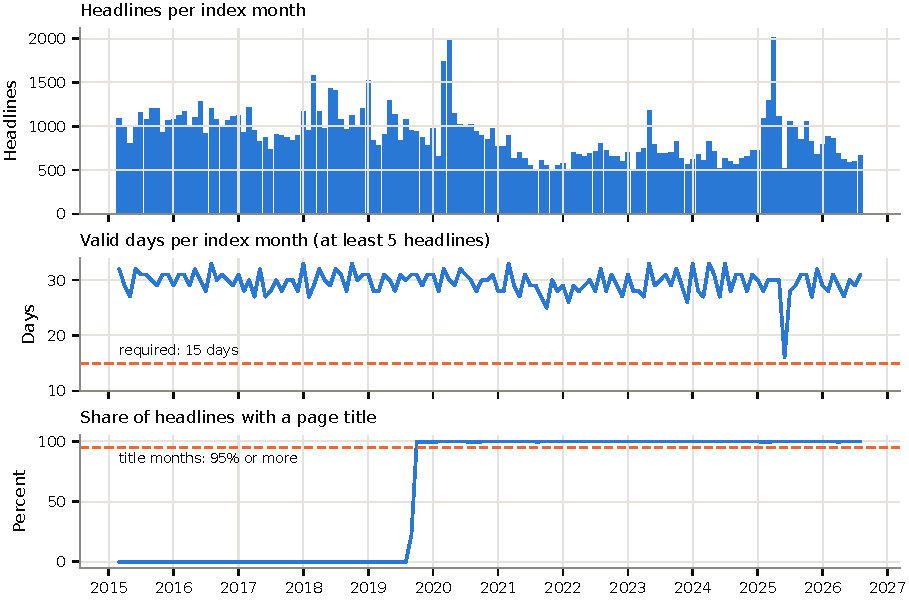
\includegraphics[width=0.92\linewidth]{figures/fig4_coverage}
  \caption{Coverage of the headline corpus by index month. Top: headlines that enter the index.
    Middle: days with enough headlines to enter the index, and the number of such days that an
    index month needs (dashed). Bottom: share of headlines with a page title, and the share
    from which a month counts as a title month in Section~\ref{sec:robust} (dashed).}
  \label{fig:coverage}
\end{figure}

\subsection{Published indices and scorer inputs}

Three published series serve as benchmarks: the Daily News Sentiment Index of the Federal
Reserve Bank of San Francisco~\cite{shapiro2022measuring}, the news-based Economic Policy
Uncertainty index for the United States~\cite{baker2016measuring} and, as a predictor of the
S\&P 500 only, the level of the consumer sentiment index. All three reach back to 1980 or
earlier, which gives a long sample of \res{E06.origins} forecasts. After an initial window of
\res{E06.window} months it leaves \res{E06.n} test months, from \res{E06.first} to
\res{E06.last}. The scorers use the
word lists of~\citet{loughran2011liability}, the Financial PhraseBank~\cite{malo2014good} and
the published FinBERT model~\cite{araci2019finbert}.

\section{Method}
\label{sec:method}

\subsection{Sentiment scorers}

A scorer maps one headline to a number that is higher for more positive text. We use four
scorers that differ in kind. The first is a lexicon, a fixed list of words tagged positive or
negative. With the finance word lists of~\citet{loughran2011liability} the score is the number
of positive words minus the number of negative words, divided by their sum, and zero if the
headline contains no listed word. Negation is not handled. The second is VADER, a
general-purpose lexicon with rules for emphasis and negation that returns one number between
$-1$ and $1$~\cite{hutto2014vader}. The third is FinBERT, a neural language model further
trained on financial text and on labelled financial sentences~\cite{araci2019finbert}. Its score
is the probability it assigns to the class positive minus the probability of the class
negative. The fourth is a classifier that we train ourselves: a logistic regression on weighted
counts of words and word pairs, fitted once to the \res{meas.labelled.clf.n} labelled sentences
of the Financial PhraseBank~\cite{malo2014good} and scored like FinBERT. In five-fold
cross-validation it classifies \res{meas.labelled.clf.acc}\% of those sentences correctly,
against \res{meas.labelled.majority}\% for always choosing the most frequent class. No scorer is
tuned on the forecast targets.

Two further indices serve as comparisons. GDELT publishes its own tone score for the whole
article, and we treat the index built from it as an external benchmark. Two large language
models are added as a secondary comparison in Section~\ref{sec:robust}.

\subsection{Index construction}

The daily index of a scorer is the mean score of the day's headlines, and a day with fewer than
five headlines is missing. The monthly index is the mean of the daily index over a window that
starts on the previous forecast date and ends the day before the current one. It needs at least
15 valid days, and all \res{corpus.months} index months meet this requirement. The primary
predictor, fixed in advance, is the composite: each of the four monthly indices is standardised
with its mean and standard deviation over the first \res{E03.window} months only, and the four
are averaged with equal weights. The composite was fixed before any experiment was run, so
that no scorer could be chosen after the results were known. Its four members are built in
different ways and need not agree. Each of them is therefore also reported on its own in
every table, with a Bonferroni adjustment, and Section~\ref{sec:results} reports how far they
agree.

\subsection{Forecast models and baselines}

For the two continuous targets we compare four linear regressions, estimated by ordinary least
squares. Let $y_{t+1}$ be the target in month $t+1$ and $x_t$ the sentiment index available on
the forecast date at the end of month $t$. M0 forecasts with the mean of $y$ so far, the
historical mean. M1 regresses $y_{t+1}$ on a constant and $y_t$, the own lag. M2 regresses
$y_{t+1}$ on a constant and $x_t$. M3 uses a constant, $y_t$ and $x_t$. M0 and M1 are the
baselines. The first asks whether the index beats a forecast that uses no predictor, the second
whether it adds to the target's own past. For the direction we use logistic regressions with
the same predictors, L0 to L3, where L0 predicts with the share of rising months so far and L1
uses the lagged excess return. A rise is predicted when the fitted probability is at least 0.5.
The published indices enter the same models in place of $x_t$.

\subsection{Evaluation}

All models are estimated again every month on an expanding window. At each forecast date the
model is fitted to all months up to that date and forecasts the next month, which is then added
to the data. The forecast month is never part of the fitting data, so accuracy is measured only
on months the model has not seen. This is what out-of-sample means here. The fit of a regression
on its own estimation sample does not show it.

The main statistic is the out-of-sample R-squared~\cite{campbell2008predicting},
\begin{equation}
  \Ros = 1 - \frac{\sum_t (y_t - \hat{y}_t)^2}{\sum_t (y_t - \bar{y}_t)^2},
\end{equation}
where $\hat{y}_t$ is the forecast of the model, $\bar{y}_t$ that of the benchmark, and the sums
run over the test months. It is the share by which the summed squared errors of the model are
smaller than those of the benchmark. It is positive when the model is more accurate, zero when
the two are equal and negative when the model is worse, with no lower bound.

A positive \Ros{} can arise by chance. M2 contains M0 as the special case in which the
coefficient on the index is zero, and M3 contains M1 in the same way; such models are called
nested. If that coefficient is truly zero, estimating it only adds noise, so the larger model
is expected to have slightly larger errors in the test months. The test
of~\citet{clark2007approximately} removes this expected penalty and then asks whether the
adjusted difference in squared errors is above zero. It is one-sided, and we use the 5\% level.
Because the test asks whether the index has predictive content, while \Ros{} measures realised
accuracy, the test can reject while \Ros{} is at or below zero.

For the direction we report three quantities. The hit rate is the share of months in which the
direction is called correctly. The test of~\citet{pesaran1992simple} asks whether the calls
match the outcomes more often than chance; it is undefined, and shown as n/a, for a model that
predicts the same direction every month. The Brier score is the mean squared error of the
predicted probability, and we compare it with that of L0 by the test
of~\citet{diebold1995comparing}. Intervals are 90\% intervals from a stationary
bootstrap~\cite{politis1994stationary}, which resamples the test months 10,000 times in blocks
with a mean length of six months, or twelve at the three-month horizon. At that horizon, where
forecasts overlap, variances use the estimator of~\citet{newey1987simple}.

\subsection{Decision rule}

The rule that maps results to an outcome was fixed before the experiments. For a continuous
target the outcome is positive if the composite beats both baselines: M2 against M0 and M3
against M1 must each have \Ros{} above zero and a Clark-West $p$-value below 0.05. The outcome
is mixed if exactly one comparison meets both conditions, and null otherwise. For the direction
the outcome is positive if the hit rate of L2 is above that of L0 and the direction test has a
$p$-value below 0.05, and null otherwise. The four individual scorers are secondary. Their
$p$-values are multiplied by four, a Bonferroni adjustment for testing four scorers, and a null
for the composite is reported as a null even if one scorer is significant. The $p$-values of
all other comparisons in the paper are not adjusted.

\subsection{Leakage controls}

Leakage is information dated after a forecast was made that enters the forecast. Three rules
prevent it. A headline is used only if the time at which GDELT recorded it is before the
forecast date. A statistic about a month is published after that month, so every monthly series
has a release lag. The policy uncertainty index is lagged one month, and so is consumer
sentiment when it predicts the S\&P 500. As its own lag, consumer sentiment enters with the
latest survey value, whose final release can fall a few days after the forecast date; the
text is still cut off at the forecast date, and Section~\ref{sec:robust} reports a variant
without that value. The daily San Francisco Fed index is cut off seven days before the
forecast date. The composite
is standardised with the first \res{E03.window} months only. Tests in the code fail if any
headline is dated on or after its forecast date or if a series has no release lag.
Figure~\ref{fig:timing} shows, for one forecast, the period that each input covers, and how the
two samples divide into months for the first estimate and test months.

\begin{figure}
  \centering
  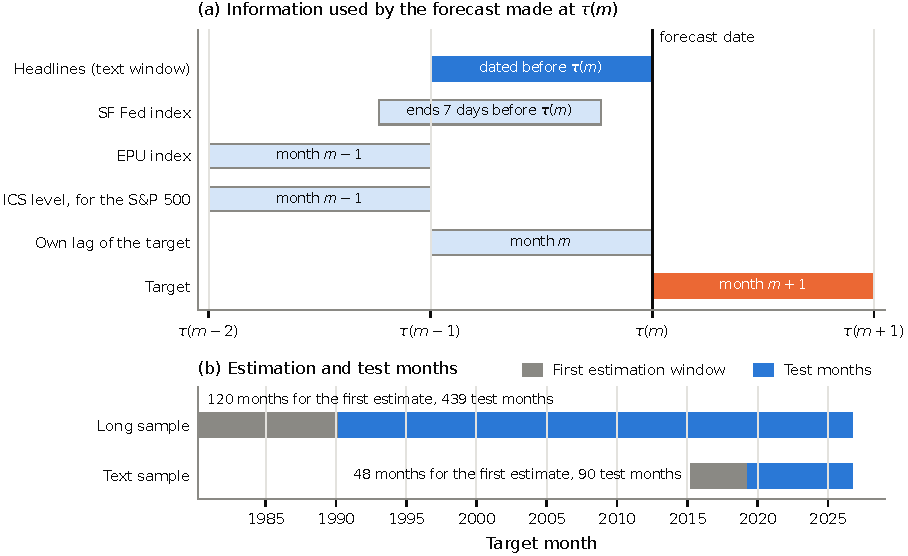
\includegraphics[width=0.95\linewidth]{figures/fig5_timing}
  \caption{Timing. (a) The inputs of the forecast made on the forecast date $\tau(m)$, the last
    trading day of month $m$, and its target. Months are drawn with equal length. For consumer
    sentiment the own lag is the latest survey value, whose final release can fall a few days
    after $\tau(m)$. (b) The months used only for the first estimate and the test months, for
    the text sample and for the long sample of the published indices.}
  \label{fig:timing}
\end{figure}

\subsection{Changes to the plan}

The plan was changed in five ways after it was fixed. First, before any request was sent to a
language model, that comparison was extended from 200 headlines per month and one model to
every headline and two models, with a split of the results at each model's training cutoff.
Second, a check of a first complete run found that the downloader stopped looking for a
replacement file after three attempts, a limit the plan does not contain, and that one
robustness variant, the stricter timing for consumer sentiment in Section~\ref{sec:robust},
was incomplete. Both were corrected, nine months of files were downloaded again, and all
experiments were run again. Third, three tables were added or split off. Fourth, settings that
the plan left open were fixed in the code, for example that a comparison needs at least 12
forecasts. Fifth, after the results were known, a simulation of the power of the main test
(Section~\ref{sec:power}) and four figures drawn from the existing results were added. Before the first complete run, a trial run on three years of the corpus had produced
the results for the published indices; no design choice was changed after it. Every outcome
under the decision rule is the same in the first complete run and in the run reported here.

\section{Results}
\label{sec:results}

\subsection{Measurement}

Before the forecasts we ask whether the index is a sound measurement (RQ4).
Table~\ref{tab:measurement} and Figure~\ref{fig:indices} summarise the checks.

The four scorers agree only moderately on single headlines. The correlation between two scorers
ranges from \res{meas.agree.headline.lm.clf} for the finance lexicon and the classifier to
\res{meas.agree.headline.lm.vader} for the two lexicons. Averaging to months raises the
agreement for some pairs and not for others: the monthly indices of the finance lexicon and of
FinBERT correlate at \res{meas.agree.month.lm.finbert}, while those of VADER and of the
classifier are almost unrelated (\res{meas.agree.month.vader.clf}).
Figure~\ref{fig:agreement} shows every pair, with the index built from GDELT's tone as a fifth
row.

\begin{figure}
  \centering
  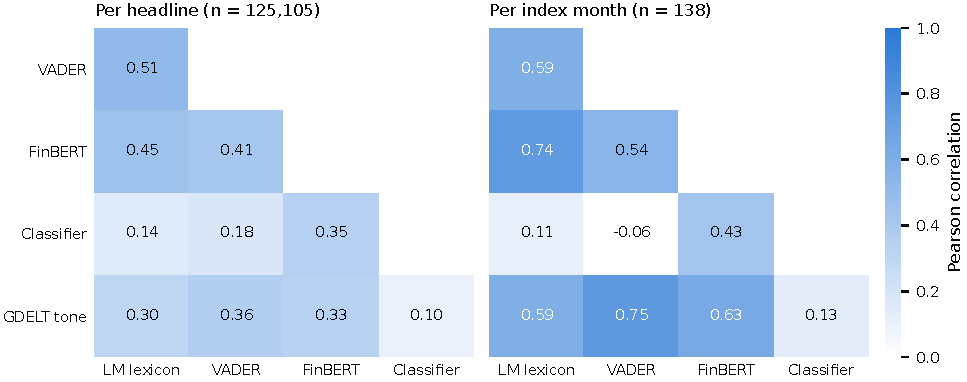
\includegraphics[width=0.92\linewidth]{figures/fig6_agreement}
  \caption{Agreement between scorers: Pearson correlation of the scores of single headlines
    (left) and of the monthly indices (right). The colour scale starts at zero.}
  \label{fig:agreement}
\end{figure}

The headline rebuilt from the web address is a close stand-in for the page title. On the
\res{meas.title.headline.n} headlines that have a title, the score of the rebuilt headline and
the score of the title correlate between \res{meas.title.headline.finbert} and
\res{meas.title.headline.lm}, depending on the scorer. The monthly indices built from the two
texts correlate at \res{meas.title.month.finbert} or more over \res{meas.title.month.n} months.

Two files a day are a small sample of each day's news, so part of the index is sampling noise.
To measure it we build the index twice, once from each of the day's two files, and correlate
the two halves; the Spearman-Brown formula then gives the reliability of the full index. It is
\res{meas.split.lm} for the finance lexicon, \res{meas.split.vader} for VADER,
\res{meas.split.finbert} for FinBERT and \res{meas.split.clf} for the classifier.

These checks bear on the composite. The classifier has the lowest reliability of the four
members, and its monthly index is almost unrelated to that of VADER, so the equal-weight mean
combines indices that share only part of their variation. We keep the composite as the
primary predictor because it was fixed in advance, and changing it now would be a choice made
with the results in view. The tables report every member next to it, and no member on its own
meets the conditions of the decision rule for any target.

\begin{figure}
  \centering
  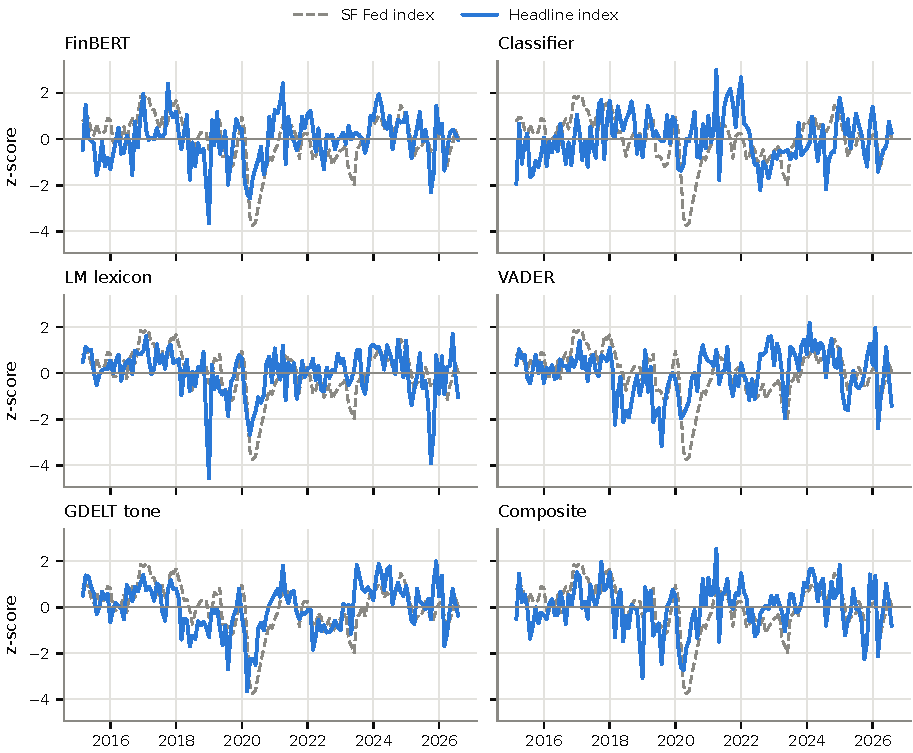
\includegraphics[width=0.88\linewidth]{figures/fig1_indices}
  \caption{Monthly sentiment indices built from the headline corpus (solid) and the Daily News
    Sentiment Index of the Federal Reserve Bank of San Francisco (dashed), \res{E03.firstorigin}
    to \res{E03.lastorigin}. Every series is standardised over the months shown.}
  \label{fig:indices}
\end{figure}

\begin{table}
  \caption{Measurement checks by index. Zero: share of headlines scored exactly zero.
    Split-half: reliability of the monthly index from the two daily files (Spearman-Brown).
    URL vs title: correlation between the scores of the rebuilt headline and of the page title,
    per headline and per month. Published series: correlation of the monthly index with the San
    Francisco Fed index and with the level of the Index of Consumer Sentiment (ICS). S\&P 500
    return: correlation with the excess return of the same and of the next month.}
  \label{tab:measurement}
  \centering
  \small
  \begin{tabular}{lrrrrrrrr}
\toprule
 &  &  & \multicolumn{2}{c}{URL vs title} & \multicolumn{2}{c}{Published series} & \multicolumn{2}{c}{S\&P 500 return} \\
\cmidrule(lr){4-5}\cmidrule(lr){6-7}\cmidrule(lr){8-9}
Index & Zero (\%) & Split-half & Headline & Month & SF Fed & ICS & Same month & Next month \\
\midrule
FinBERT & 0.0 & 0.79 & 0.86 & 0.96 & 0.41 & $-$0.02 & 0.20 & $-$0.09 \\
Classifier & 0.0 & 0.63 & 0.87 & 0.97 & 0.13 & 0.14 & 0.11 & $-$0.07 \\
LM lexicon & 62.6 & 0.86 & 0.92 & 0.98 & 0.49 & 0.15 & 0.07 & $-$0.15 \\
VADER & 38.2 & 0.87 & 0.90 & 0.99 & 0.37 & $-$0.11 & 0.17 & $-$0.14 \\
GDELT tone & 4.1 & 0.92 & n/a & n/a & 0.60 & 0.01 & 0.18 & $-$0.13 \\
Composite & n/a & n/a & n/a & n/a & 0.48 & 0.05 & 0.19 & $-$0.15 \\
\bottomrule
\end{tabular}

\end{table}

\begin{table}
  \caption{Accuracy and macro-F1 on the Financial PhraseBank with three classes. The classifier
    is evaluated by five-fold cross-validation. FinBERT was trained on these sentences. The
    scores of the two lexicons are turned into classes at $-0.05$ and $0.05$.}
  \label{tab:labelled}
  \centering
  \begin{tabular}{lrr}
\toprule
Scorer & Accuracy (\%) & Macro-F1 (\%) \\
\midrule
Classifier (5-fold) & 76.2 & 66.8 \\
LM lexicon & 63.2 & 51.1 \\
VADER & 54.3 & 48.9 \\
FinBERT (in sample) & 88.9 & 88.2 \\
Majority class & 59.4 & n/a \\
\bottomrule
\end{tabular}

\end{table}

The composite correlates at \res{meas.corr.composite.sffed} with the San Francisco Fed index in
levels and at \res{meas.corr.composite.dsffed} in monthly changes (Figure~\ref{fig:indices}).
Its correlation with the S\&P 500 excess return is \res{meas.corr.composite.retsame} for the
same month and \res{meas.corr.composite.retnext} for the next month. On the labelled sentences
(Table~\ref{tab:labelled}) the two lexicons classify \res{meas.labelled.lm.acc}\% and
\res{meas.labelled.vader.acc}\% correctly. FinBERT reaches \res{meas.labelled.finbert.acc}\%, but
it was trained on these sentences.

\subsection{S\&P 500 return and direction}

Table~\ref{tab:sp500return} reports the forecasts of the S\&P 500 excess return (RQ1). The own
lag does not help: M1 has a larger squared error than the historical mean, with an \Ros{} of
\res{E03.ar.r2}\%. Adding the composite to the historical mean gives an \Ros{} of
\res{E03.composite.m0.r2}\%, with a 90\% interval from \res{E03.composite.m0.lo}\% to
\res{E03.composite.m0.hi}\% and a Clark-West $p$-value of \res{E03.composite.m0.p}. Adding it to
the own-lag model gives \res{E03.composite.m1.r2}\% (interval \res{E03.composite.m1.lo}\% to
\res{E03.composite.m1.hi}\%, $p = \res{E03.composite.m1.p}$). Neither comparison meets the
conditions of the rule, so the outcome is \res{E03.outcome}.

No individual scorer changes this. Their \Ros{} against the historical mean lies between
\res{E03.clf.m0.r2}\% for the classifier and \res{E03.vader.m0.r2}\% for VADER, and the smallest
$p$-value before the Bonferroni adjustment is \res{E03.lm.m0.p}. The index built from GDELT's
own tone gives \res{E03.gdelt.m0.r2}\%. Figure~\ref{fig:cssed} shows when the composite gains
and loses against each benchmark. The gain is not steady. Against the historical mean the
largest loss in a single month falls in \res{E03.cssed.worst} and the largest gain in
\res{E03.cssed.best}, and that one month supplies \res{E03.cssed.bestvalue} of the total gain
of \res{E03.cssed.total} in squared percentage points. Figure~\ref{fig:r2} collects the point
estimates and the intervals.

\begin{figure}
  \centering
  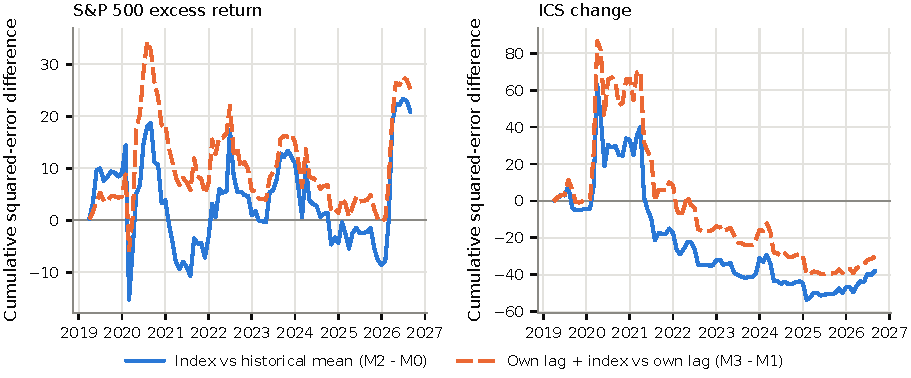
\includegraphics[width=0.92\linewidth]{figures/fig2_cssed}
  \caption{Cumulative difference in squared forecast errors over the test months, benchmark
    minus model with the composite index. A rising line means that the model with the index was
    more accurate than its benchmark in that month. Left: S\&P 500 excess return. Right: change
    in the Index of Consumer Sentiment (ICS).}
  \label{fig:cssed}
\end{figure}

\begin{figure}
  \centering
  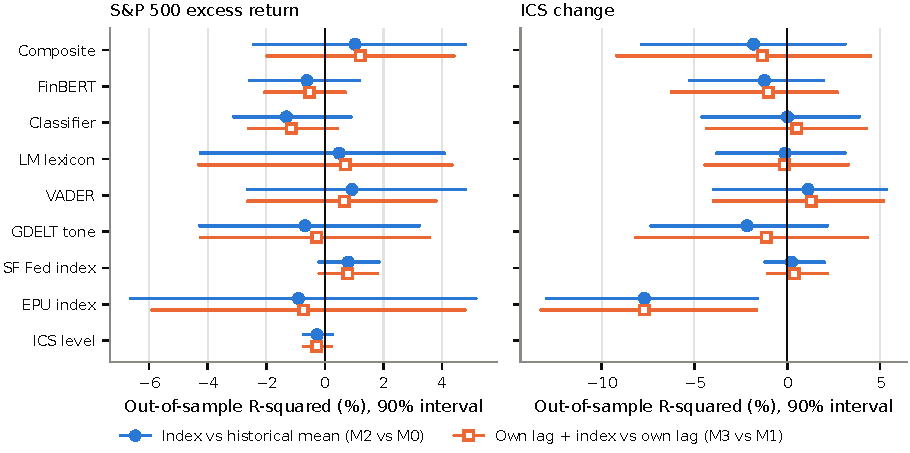
\includegraphics[width=0.92\linewidth]{figures/fig3_r2}
  \caption{Out-of-sample R-squared with 90\% bootstrap intervals, by predictor, on the
    \res{E03.n} test months of the text sample. The models with published indices are estimated
    on data from 1980.}
  \label{fig:r2}
\end{figure}

\begin{table}
  \caption{One-month-ahead forecasts of the S\&P 500 excess return. $R^2_{OS}$ is the
    out-of-sample R-squared in percent, for a model with the predictor against the historical
    mean (M0) and for a model with the own lag and the predictor against the own-lag model
    (M1). Intervals are 90\% bootstrap intervals. $p$ is the one-sided Clark-West $p$-value and
    $p$ adj.\ its Bonferroni adjustment for the four individual scorers. Upper block: text
    indices, \res{E03.n} test months. Lower blocks: published indices.}
  \label{tab:sp500return}
  \centering
  \resizebox{\linewidth}{!}{\begin{tabular}{lrcrrrcrr}
\toprule
Predictor & $R^2_{OS}$ vs M0 (\%) & 90\% interval & $p$ & $p$ adj. & $R^2_{OS}$ vs M1 (\%) & 90\% interval & $p$ & $p$ adj. \\
\midrule
Composite & 1.03 & [$-$2.44, 4.80] & 0.149 &  & 1.21 & [$-$1.97, 4.41] & 0.115 &  \\
FinBERT & $-$0.62 & [$-$2.56, 1.18] & 0.542 & 1.000 & $-$0.53 & [$-$2.06, 0.69] & 0.627 & 1.000 \\
Classifier & $-$1.31 & [$-$3.12, 0.89] & 0.737 & 1.000 & $-$1.15 & [$-$2.59, 0.43] & 0.817 & 1.000 \\
LM lexicon & 0.49 & [$-$4.25, 4.07] & 0.134 & 0.534 & 0.70 & [$-$4.31, 4.33] & 0.129 & 0.518 \\
VADER & 0.92 & [$-$2.62, 4.80] & 0.170 & 0.681 & 0.66 & [$-$2.63, 3.79] & 0.217 & 0.866 \\
GDELT tone & $-$0.68 & [$-$4.27, 3.23] & 0.392 &  & $-$0.28 & [$-$4.24, 3.57] & 0.364 &  \\
\midrule
\multicolumn{9}{l}{Published indices and their benchmarks, estimated from 1980: same 90 test months} \\
SF Fed index & 0.80 & [$-$0.20, 1.84] & 0.076 &  & 0.78 & [$-$0.19, 1.80] & 0.078 &  \\
EPU index & $-$0.90 & [$-$6.62, 5.15] & 0.040 &  & $-$0.73 & [$-$5.90, 4.78] & 0.042 &  \\
ICS level & $-$0.26 & [$-$0.74, 0.27] & 0.780 &  & $-$0.28 & [$-$0.72, 0.23] & 0.806 &  \\
\midrule
\multicolumn{9}{l}{Published indices and their benchmarks, estimated from 1980: long sample, 439 test months} \\
SF Fed index & $-$0.79 & [$-$1.98, 0.36] & 0.516 &  & $-$0.72 & [$-$1.86, 0.33] & 0.496 &  \\
EPU index & $-$0.34 & [$-$3.23, 2.67] & 0.002 &  & $-$0.27 & [$-$3.04, 2.55] & 0.002 &  \\
ICS level & $-$0.55 & [$-$1.10, $-$0.03] & 0.915 &  & $-$0.54 & [$-$1.04, $-$0.07] & 0.931 &  \\
\bottomrule
\end{tabular}
}
\end{table}

\begin{table}
  \caption{One-month-ahead forecasts of the direction of the S\&P 500 from logistic models. Hit
    rate: share of test months with the direction called correctly. Predicted up: share of
    months in which a rise is predicted. PT $p$: Pesaran-Timmermann test, n/a when the model
    predicts the same direction every month. Brier: mean squared error of the predicted
    probability. DM $p$: Diebold-Mariano test of the Brier score against the L0 of the same
    block.}
  \label{tab:sp500direction}
  \centering
  \resizebox{\linewidth}{!}{\begin{tabular}{lrcrrrrr}
\toprule
Predictor & Hit rate (\%) & 90\% interval & Predicted up (\%) & PT $p$ & PT $p$ adj. & Brier & DM $p$ vs L0 \\
\midrule
Base rate (L0) & 63.3 & [56.7, 70.0] & 100.0 & n/a &  & 0.2369 & n/a \\
Lagged return (L1) & 62.2 & [55.6, 68.9] & 98.9 & 0.779 &  & 0.2420 & 0.134 \\
\midrule
Composite & 63.3 & [56.7, 70.0] & 100.0 & n/a &  & 0.2377 & 0.818 \\
FinBERT & 63.3 & [56.7, 70.0] & 100.0 & n/a & n/a & 0.2417 & 0.048 \\
Classifier & 63.3 & [56.7, 70.0] & 100.0 & n/a & n/a & 0.2401 & 0.094 \\
LM lexicon & 63.3 & [56.7, 70.0] & 100.0 & n/a & n/a & 0.2407 & 0.530 \\
VADER & 63.3 & [56.7, 70.0] & 100.0 & n/a & n/a & 0.2372 & 0.967 \\
GDELT tone & 63.3 & [56.7, 70.0] & 100.0 & n/a &  & 0.2392 & 0.663 \\
\midrule
\multicolumn{8}{l}{Published indices and their benchmarks, estimated from 1980: same 90 test months} \\
Base rate (L0) & 63.3 & [56.7, 70.0] & 100.0 & n/a &  & 0.2327 & n/a \\
Lagged return (L1) & 63.3 & [56.7, 70.0] & 100.0 & n/a &  & 0.2340 & 0.465 \\
SF Fed index & 63.3 & [56.7, 70.0] & 100.0 & n/a &  & 0.2321 & 0.606 \\
EPU index & 63.3 & [56.7, 70.0] & 100.0 & n/a &  & 0.2392 & 0.533 \\
ICS level & 63.3 & [56.7, 70.0] & 100.0 & n/a &  & 0.2339 & 0.049 \\
\midrule
\multicolumn{8}{l}{Published indices and their benchmarks, estimated from 1980: long sample, 439 test months} \\
Base rate (L0) & 63.8 & [59.7, 67.9] & 100.0 & n/a &  & 0.2323 & n/a \\
Lagged return (L1) & 63.8 & [59.7, 67.7] & 100.0 & n/a &  & 0.2329 & 0.363 \\
SF Fed index & 62.6 & [58.8, 66.7] & 96.1 & 0.532 &  & 0.2353 & 0.126 \\
EPU index & 63.1 & [59.0, 67.0] & 98.9 & 0.776 &  & 0.2340 & 0.622 \\
ICS level & 63.8 & [59.7, 67.7] & 100.0 & n/a &  & 0.2333 & 0.139 \\
\bottomrule
\end{tabular}
}
\end{table}

Table~\ref{tab:sp500direction} reports the direction forecasts. Every model that uses a text
index alone predicts a rise in each of the \res{E04.composite.n} test months. Its hit rate
therefore equals the base rate of \res{E04.composite.base}\%, and the direction test is
undefined. Figure~\ref{fig:probability} shows the fitted probabilities behind these calls: for
the composite and for every individual index they stay at or above the threshold of 0.5 in
all test months. The predicted probabilities are no more accurate than the base rate: the Brier score
of the composite is \res{E04.composite.brier}, against \res{E04.composite.brierbase} for L0. The
outcome is \res{E04.outcome}.

\begin{figure}
  \centering
  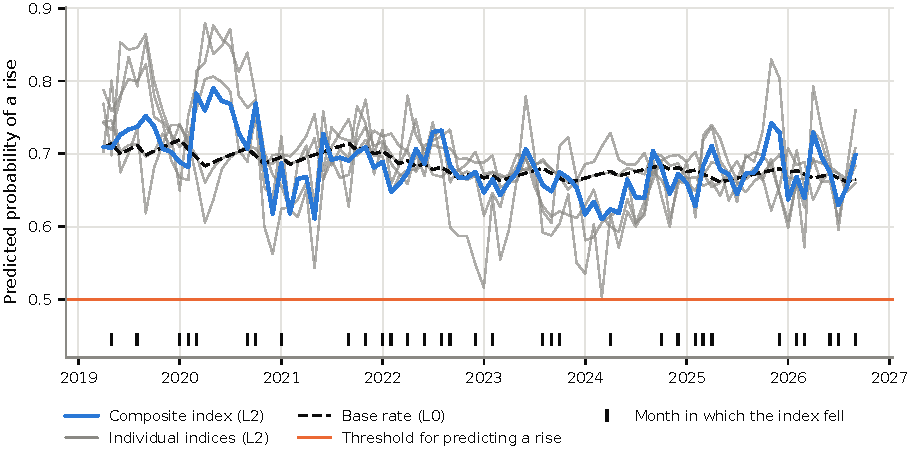
\includegraphics[width=0.92\linewidth]{figures/fig7_probability}
  \caption{Predicted probability that the S\&P 500 rises in the next month, from the logistic
    models with one text index (L2) and from the base-rate model (L0), over the
    \res{E04.composite.n} test months. A rise is predicted when the probability is at least
    0.5. The marks at the bottom show the months in which the index fell.}
  \label{fig:probability}
\end{figure}

\subsection{Consumer sentiment}

Table~\ref{tab:ics} reports the forecasts of the change in consumer sentiment (RQ2). The own
lag is again worse than the historical mean, with an \Ros{} of \res{E05.ar.r2}\%. The composite
improves on neither baseline. Its \Ros{} is \res{E05.composite.m0.r2}\% against the historical
mean ($p = \res{E05.composite.m0.p}$) and \res{E05.composite.m1.r2}\% when it is added to the own
lag ($p = \res{E05.composite.m1.p}$). The outcome is \res{E05.outcome}. Among the individual
scorers VADER has the largest \Ros{}, \res{E05.vader.m0.r2}\%, with a $p$-value of
\res{E05.vader.m0.p} before the adjustment and \res{E05.vader.m0.padj} after it.

\begin{table}
  \caption{One-month-ahead forecasts of the change in the Index of Consumer Sentiment. Columns
    and blocks as in Table~\ref{tab:sp500return}.}
  \label{tab:ics}
  \centering
  \resizebox{\linewidth}{!}{\begin{tabular}{lrcrrrcrr}
\toprule
Predictor & $R^2_{OS}$ vs M0 (\%) & 90\% interval & $p$ & $p$ adj. & $R^2_{OS}$ vs M1 (\%) & 90\% interval & $p$ & $p$ adj. \\
\midrule
Composite & $-$1.81 & [$-$7.85, 3.10] & 0.450 &  & $-$1.35 & [$-$9.19, 4.49] & 0.387 &  \\
FinBERT & $-$1.23 & [$-$5.25, 1.92] & 0.483 & 1.000 & $-$1.02 & [$-$6.24, 2.71] & 0.441 & 1.000 \\
Classifier & 0.01 & [$-$4.58, 3.87] & 0.331 & 1.000 & 0.51 & [$-$4.34, 4.25] & 0.239 & 0.956 \\
LM lexicon & $-$0.12 & [$-$3.80, 3.11] & 0.287 & 1.000 & $-$0.16 & [$-$4.42, 3.29] & 0.318 & 1.000 \\
VADER & 1.13 & [$-$3.96, 5.31] & 0.120 & 0.481 & 1.29 & [$-$3.98, 5.19] & 0.108 & 0.431 \\
GDELT tone & $-$2.16 & [$-$7.34, 2.16] & 0.469 &  & $-$1.12 & [$-$8.17, 4.29] & 0.368 &  \\
\midrule
\multicolumn{9}{l}{Published indices and their benchmarks, estimated from 1980: same 90 test months} \\
SF Fed index & 0.23 & [$-$1.21, 1.99] & 0.337 &  & 0.37 & [$-$1.06, 2.15] & 0.300 &  \\
EPU index & $-$7.69 & [$-$12.97, $-$1.59] & 0.693 &  & $-$7.70 & [$-$13.25, $-$1.65] & 0.693 &  \\
\midrule
\multicolumn{9}{l}{Published indices and their benchmarks, estimated from 1980: long sample, 439 test months} \\
SF Fed index & $-$0.55 & [$-$2.61, 1.23] & 0.262 &  & $-$0.58 & [$-$2.61, 1.19] & 0.269 &  \\
EPU index & $-$1.11 & [$-$4.13, 1.79] & 0.086 &  & $-$1.11 & [$-$4.20, 1.82] & 0.086 &  \\
\bottomrule
\end{tabular}
}
\end{table}

\subsection{Published indices}

The lower blocks of Tables~\ref{tab:sp500return} to~\ref{tab:ics} repeat the exercise with the
published indices (RQ3). These models and their benchmarks are estimated on data from 1980, so
their baselines differ from those of the text models, which start in 2015. Over the long sample
of \res{E06.n} test months none of the three indices lowers the squared error for the S\&P 500
return. The \Ros{} against the historical mean is \res{E06.long.sp.sffed.m0.r2}\% for the San
Francisco Fed index, \res{E06.long.sp.epu.m0.r2}\% for the policy uncertainty index and
\res{E06.long.sp.icslevel.m0.r2}\% for the level of consumer sentiment. For the policy
uncertainty index the Clark-West test rejects ($p = \res{E06.long.sp.epu.m0.p}$) although its
\Ros{} is negative, the case described in Section~\ref{sec:method}. For consumer sentiment the
San Francisco Fed index gives \res{E06.long.ics.sffed.m0.r2}\% against the historical mean and
\res{E06.long.ics.sffed.m1.r2}\% when it is added to the own lag. On the \res{E06.text.n} months
of the text sample the San Francisco Fed index gives \res{E06.text.sp.sffed.m0.r2}\% for the
S\&P 500 return ($p = \res{E06.text.sp.sffed.m0.p}$) and \res{E06.text.ics.sffed.m0.r2}\% for
consumer sentiment ($p = \res{E06.text.ics.sffed.m0.p}$).

Table~\ref{tab:incremental} asks whether the composite adds to models that already contain the
published indices. Added to a model with the San Francisco Fed index it gives an \Ros{} of
\res{E07.sp.sffed.r2}\% for the S\&P 500 return. For consumer sentiment, added to the own lag
and the San Francisco Fed index, it gives \res{E07.ics.sffed.r2}\% ($p = \res{E07.ics.sffed.p}$),
and added to the own lag and the lagged S\&P 500 return it gives \res{E07.ics.lagret.r2}\%.

\begin{table}
  \caption{The composite index added to models that already contain other predictors.
    $R^2_{OS}$ compares the model with the composite against the same model without it, on
    \res{E07.sp.sffed.n} test months.}
  \label{tab:incremental}
  \centering
  \resizebox{\linewidth}{!}{\begin{tabular}{llrcr}
\toprule
Target & Benchmark holds & $R^2_{OS}$ vs benchmark (\%) & 90\% interval & $p$ \\
\midrule
S\&P 500 excess return & SF Fed index & $-$0.79 & [$-$3.25, 1.86] & 0.594 \\
S\&P 500 excess return & SF Fed index, EPU index, ICS level & $-$0.94 & [$-$2.74, 1.34] & 0.660 \\
\midrule
ICS change & own lag, SF Fed index & 0.46 & [$-$9.00, 7.39] & 0.152 \\
ICS change & own lag, SF Fed index, EPU index & 0.30 & [$-$8.92, 6.65] & 0.178 \\
ICS change & own lag, lagged S\&P 500 return & $-$1.27 & [$-$4.24, 1.28] & 0.617 \\
\bottomrule
\end{tabular}
}
\end{table}

\section{Robustness and limitations}
\label{sec:robust}

\subsection{Robustness}

Table~\ref{tab:robustness} repeats the three main experiments under other choices. With an
initial window of 36 or 60 months, or a rolling window of 48 months, the \Ros{} of the composite
for the S\&P 500 return is \res{E08.initial36.sp.m0.r2}\%, \res{E08.initial60.sp.m0.r2}\% and
\res{E08.rolling48.sp.m0.r2}\%, and no outcome changes. No outcome changes either when the index
enters in first differences, when the monthly index weights headlines and not days, or when the
index is built from page titles on the \res{E09.title.n} test months that have them. With the
raw log return or a simple excess return as the target, the \Ros{} is \res{E10.raw.m0.r2}\% and
\res{E10.simple.m0.r2}\%. For consumer sentiment a stricter variant, in which the latest survey
value is assumed unknown on the forecast date, gives \res{E10.strict.m1.r2}\% when the composite
is added to the own lag.

\begin{table}
  \caption{Robustness of the composite index. $n$: number of test months. $R^2_{OS}$ and hit
    rates are in percent. Hit rate / base: hit
    rate of the logistic model with the composite and of the base-rate model. Title months:
    index months in which at least 95\% of the headlines have a page title. ICS: Index of
    Consumer Sentiment.}
  \label{tab:robustness}
  \centering
  \footnotesize\setlength{\tabcolsep}{4pt}
  \begin{tabular}{lrrrrrrrr}
\toprule
 &  & \multicolumn{3}{c}{S\&P 500} & \multicolumn{4}{c}{ICS change} \\
\cmidrule(lr){3-5}\cmidrule(lr){6-9}
Variant & $n$ & $R^2_{OS}$ vs M0 & $p$ & Hit rate / base & $R^2_{OS}$ vs M0 & $p$ & $R^2_{OS}$ vs M1 & $p$ \\
\midrule
Initial window 36 & 102 & 0.75 & 0.142 & 64.7 / 65.7 & $-$1.35 & 0.354 & $-$0.43 & 0.264 \\
Initial window 60 & 78 & 2.14 & 0.062 & 64.1 / 64.1 & $-$2.66 & 0.528 & $-$2.94 & 0.536 \\
Rolling window 48 & 90 & 0.97 & 0.153 & 63.3 / 63.3 & $-$2.34 & 0.371 & $-$1.33 & 0.301 \\
\midrule
Index in first differences & 89 & $-$1.72 & 0.889 & 61.8 / 62.9 & 1.63 & 0.091 & 1.32 & 0.092 \\
Headline-weighted index & 90 & $-$0.06 & 0.253 & 63.3 / 63.3 & $-$1.53 & 0.362 & $-$1.24 & 0.324 \\
Page-title index (title months) & 47 & 2.14 & 0.175 & 63.8 / 63.8 & 0.53 & 0.284 & $-$1.17 & 0.533 \\
URL-headline index (title months) & 47 & 1.59 & 0.191 & 63.8 / 63.8 & $-$0.18 & 0.343 & $-$1.73 & 0.619 \\
\midrule
Raw log return & 90 & 0.92 & 0.160 &  &  &  &  &  \\
Simple excess return & 90 & 1.33 & 0.117 &  &  &  &  &  \\
ICS own lag, release lag 1 & 88 &  &  &  & $-$2.80 & 0.600 & $-$1.90 & 0.373 \\
\midrule
Three-month horizon & 86 & 5.69 & 0.049 &  & 0.85 & 0.181 & $-$0.30 & 0.449 \\
\bottomrule
\end{tabular}

\end{table}

At a three-month horizon the result for the S\&P 500 differs. The composite gives an \Ros{} of
\res{E11.sp.m0.r2}\% against the historical mean, with an interval from \res{E11.sp.m0.lo}\% to
\res{E11.sp.m0.hi}\% and a $p$-value of \res{E11.sp.m0.p}, and \res{E11.sp.m1.r2}\% when it is
added to the own lag ($p = \res{E11.sp.m1.p}$). Under the rule this outcome is
\res{E11.sp.outcome}. The \res{E11.n} test months of this experiment overlap, and the plan
lists the three-month horizon as a secondary analysis. For consumer sentiment the outcome at
three months is \res{E11.ics.outcome}.

\subsection{Power of the main test}
\label{sec:power}

The analysis in this subsection was not part of the plan. It was designed after the outcomes
were known and has no outcome under the decision rule. It asks how large the predictive
content of the composite would have to be for the main test to find it on \res{E03.n} test
months. We hold the composite at its observed values and simulate the target for a range of
true R-squared values, where the true R-squared is the share of the variance of the target
that the index explains in the simulated data. The noise is drawn with replacement from the
standardised observed target, which keeps its tails. For each value, \res{power.reps}
simulated samples go through the same expanding-window forecasts of M0 and M2 and the same
Clark-West test as the data. Power is the share of samples in which M2 meets both conditions
of the decision rule against M0: an \Ros{} above zero and a $p$-value below 0.05.

For the S\&P 500 excess return the power is \res{power.sp.at1}\% at a true R-squared of 1\%,
\res{power.sp.at2}\% at 2\% and \res{power.sp.at5}\% at 5\%. It reaches 50\% at a true
R-squared of \res{power.sp.r50}\% and 80\% at \res{power.sp.r80}\%. When the index has no
predictive content, \res{power.sp.zero}\% of the samples meet both conditions. For the change
in consumer sentiment the power also reaches 80\% at \res{power.ics.r80}\%; the two
simulations differ only in the distribution of the noise. The simulation covers the
comparison with the historical mean at the one-month horizon. It assumes a linear relation
that is constant over the sample and noise that is independent across months.

\subsection{Language models as scorers}

%% The LLM scorer runs only with an API key, so its table may not exist.
\IfFileExists{tables/tab7_llm.tex}{%
\begin{table}
  \caption{The sentiment index of a large language model in the forecasting models, by model.
    The second and third row of each block split the test months by whether the whole text
    window lies after the month in which the training data of the model end, as stated by its
    provider. $R^2_{OS}$ and hit rates are in percent. n/a: fewer than 12 forecasts.}
  \label{tab:llm}
  \centering
  \footnotesize\setlength{\tabcolsep}{4pt}
  \begin{tabular}{lrrrrrrrr}
\toprule
 &  & \multicolumn{3}{c}{S\&P 500} & \multicolumn{4}{c}{ICS change} \\
\cmidrule(lr){3-5}\cmidrule(lr){6-9}
Model and test months & $n$ & $R^2_{OS}$ vs M0 & $p$ & Hit rate / base & $R^2_{OS}$ vs M0 & $p$ & $R^2_{OS}$ vs M1 & $p$ \\
\midrule
claude-haiku-4-5, all test months & 90 & $-$1.51 & 0.459 & 62.2 / 63.3 & 0.37 & 0.185 & 0.71 & 0.183 \\
\quad after the cutoff month (2025-07) & 12 & 4.31 & 0.216 & 50.0 / 50.0 & 13.38 & 0.029 & 11.41 & 0.019 \\
\quad other test months & 78 & $-$1.98 & 0.511 & 64.1 / 65.4 & $-$0.64 & 0.301 & $-$0.05 & 0.262 \\
\midrule
claude-sonnet-5-5, all test months & 90 & $-$1.86 & 0.637 & 62.2 / 63.3 & 0.29 & 0.193 & 0.72 & 0.184 \\
\quad after the cutoff month (2026-06) & 1 & n/a & n/a & n/a & n/a & n/a & n/a & n/a \\
\quad other test months & 89 & $-$1.80 & 0.628 & 62.9 / 64.0 & 0.09 & 0.213 & 0.58 & 0.196 \\
\bottomrule
\end{tabular}

\end{table}}{}

Table~\ref{tab:llm} reports a secondary comparison in which the scorer is a large language
model. Two commercial models, \texttt{\res{E12.a.model}} and \texttt{\res{E12.b.model}}, label
each headline with an integer from $-2$ to $2$, and the index is built as for the other
scorers. This index is outside the composite and the decision rule, and its $p$-values are not
adjusted. Over all test months the index of neither model improves on the baselines for the
S\&P 500 return, with an \Ros{} of \res{E12.a.all.sp.m0.r2}\% for the first model and
\res{E12.b.all.sp.m0.r2}\% for the second. For consumer sentiment, added to the own lag, the
two give \res{E12.a.all.ics.m1.r2}\% ($p = \res{E12.a.all.ics.m1.p}$) and
\res{E12.b.all.ics.m1.r2}\% ($p = \res{E12.b.all.ics.m1.p}$).

A language model may have been trained on text written after the headlines it
scores~\cite{glasserman2023assessing}. The training data of the first model end in
\res{E12.a.cutoff} according to its provider, and \res{E12.a.post.months} test months have a
text window that lies wholly after that month. On these months its index gives
\res{E12.a.post.sp.m0.r2}\% for the S\&P 500 return ($p = \res{E12.a.post.sp.m0.p}$) and
\res{E12.a.post.ics.m1.r2}\% for consumer sentiment added to the own lag, with an interval from
\res{E12.a.post.ics.m1.lo}\% to \res{E12.a.post.ics.m1.hi}\% and a $p$-value of
\res{E12.a.post.ics.m1.p}. Three facts qualify this number. The sample is the smallest that our
code evaluates. The forecasting models are still estimated on index values from before the
cutoff. The comparison is one of many in this paper. For the second model only
\res{E12.b.post.months} test month has a text window wholly after the cutoff, so the comparison
cannot be made.

\subsection{Limitations}

The test covers \res{E03.n} months, which include the fall and recovery of the market in March
and April 2020. A sample of this size has low power. By the simulation of Section~\ref{sec:power}
the test reaches a power of 80\% only from a true R-squared of \res{power.sp.r80}\%, which is
far above the small values that can matter to an investor~\cite{campbell2008predicting}, and
that simulation was itself designed after the results were known. Every headline number
therefore comes with an interval. The study covers one country, one stock index and one survey series. The
S\&P 500 series is a price index without dividends, and the release dates of the consumer
sentiment survey were not verified by machine.

The corpus has five limits. Headlines are rebuilt from web addresses and are not the titles
that readers saw. Two files a day cover a small part of each day's news. The set of sources
changes over the sample: \res{corpus.mix.share}\% of the headlines of \res{corpus.mix.yearb}
come from domains that also appear in \res{corpus.mix.yeara}, and \res{corpus.mix.top20} of the
20 largest domains are the same in both years. The archive has no readable file for
\res{corpus.daysnofile} days in June and July 2025, so the index month of
\res{corpus.validdays.minmonth} rests on \res{corpus.validdays.min} days. The list of economy
and market terms was fixed by hand in 2026, after the sample period, and was not validated
against human labels.

Several scorers and targets are tested. One primary predictor was fixed in advance and the
four individual scorers carry a Bonferroni adjustment, but the $p$-values of the tone index,
the published indices, the robustness checks and the language models are unadjusted. The
published indices are used as downloaded in October 2026, and revisions of their history were
not examined. For the language models, one request holds up to 40 headlines, so a label can be
produced next to headlines dated after a forecast date, and the training cutoffs are statements
of the provider that we did not check. That comparison is also the only part of the study that
needs a paid service.

\section{Conclusion}
\label{sec:conclusion}

We tested whether sentiment measured from free news headlines improves one-month-ahead
forecasts of the S\&P 500 and of consumer sentiment, with the plan and the decision rule fixed
in advance. Under that rule the outcome is null for the S\&P 500 excess return, for its
direction and for the change in consumer sentiment. The measurement checks describe an index
that is reliable given the sampling, with a split-half reliability between
\res{meas.split.clf} and \res{meas.split.vader}, that agrees with an index built from page
titles and that correlates with a published news sentiment index. Published indices do not
lower the squared error of the S\&P 500 forecasts over \res{E06.n} test months either.

The null has a limited meaning. It agrees with the finding that most predictors of the
aggregate stock return fail out of sample~\cite{welch2008comprehensive,goyal2024comprehensive}.
It does not show that news sentiment carries no information. The 90\% interval for the S\&P
500 return includes zero and also values that would be large by the standards of that
literature, in which a small out-of-sample R-squared can matter to an
investor~\cite{campbell2008predicting}, and \res{E03.n} test months cannot separate the two. The power simulation says the same from
the other side: the test finds a true R-squared of 1\% in \res{power.sp.at1}\% of simulated
samples and needs \res{power.sp.r80}\% for a power of 80\%. The null speaks against a large
effect and leaves a small one open.
The measurement checks narrow the reading in one respect: sampling noise does not dominate
the index, and its use of web addresses in place of titles changes little.

Two results fall outside the null. At a three-month horizon the outcome for the S\&P 500 return
is \res{E11.sp.outcome}, and the index of one language model lowers the squared error for
consumer sentiment on the \res{E12.a.post.months} months after its training cutoff. Both rest
on small or overlapping samples and neither is the primary test, so we report them as
candidates for a future test fixed in advance and not as findings. Within the same design the
natural extensions are a larger share of each day's news, the text of the articles, and the
daily horizon at which earlier studies report effects~\cite{tetlock2007giving,garcia2013sentiment}.
The study reruns from free data with one command, so the test can be repeated as months are
added to the sample.

\section*{Acknowledgements}
This research received no specific funding.

%% Disclosure of AI use: Wiley asks for it in the acknowledgements when AI assists with
%% drafting, editing or formatting. Every sentence has to be true when the paper is submitted.
\paragraph{Use of AI tools.}
During the preparation of this work, the author used Claude (Anthropic). The tool was used to
suggest related literature during background research, to propose a rudimentary outline of the
sections of the paper and to organise the code repository that accompanies the paper. It was not
used to generate text for the paper: all text was written by the author. The author takes full
responsibility for the publication's content. The two language models evaluated as sentiment
scorers in Section~\ref{sec:robust} are objects of study and were not used for writing.

\section*{Statements}

\paragraph{Data availability.}
The data come from the public sources named in Section~\ref{sec:data}. The code, the result
files behind every table and figure, and the command that reruns the study from raw downloads
are available at \url{https://github.com/vignesh-nagarajan-vn/SentCast}. The language model
labels used in Section~\ref{sec:robust} are reproduced from cached files, because the model
\texttt{\res{E12.a.model}} may no longer be served. These labels are not part of the
repository and are available from the author on request.

\paragraph{Funding.}
This research received no specific funding.

\paragraph{Conflict of interest.}
The author declares no conflict of interest.

\bibliography{references}

\end{document}
